%%%%%%%%%%%%%%%%%%%%%%%%%%%%%%%%%%%%%%%%%
% Beamer Presentation
% LaTeX Template
% Version 1.0 (10/11/12)
%
% This template has been downloaded from:
% http://www.LaTeXTemplates.com
%
% License:
% CC BY-NC-SA 3.0 (http://creativecommons.org/licenses/by-nc-sa/3.0/)
%
%%%%%%%%%%%%%%%%%%%%%%%%%%%%%%%%%%%%%%%%%

%----------------------------------------------------------------------------------------
%	PACKAGES AND THEMES
%----------------------------------------------------------------------------------------

\documentclass[aspectratio=169, hyperref={colorlinks=true,pdfpagelabels=false,linkcolor=black}, xcolor=dvipsnames,10pt]{beamer}
\hypersetup{pdftex=true, colorlinks=true, breaklinks=true, linkcolor=black, menucolor=blue, pagecolor=blue, urlcolor=cyan}


\usepackage{graphicx} % Allows including images
\usepackage{booktabs} % Allows the use of \toprule, \midrule and \bottomrule in tables
\usepackage{xcolor, color}% ,colortbl}
\usepackage{tikz} % nalipour
\usetikzlibrary{tikzmark} % nalipour
\usepackage{hyperref}
\usetikzlibrary{shapes,arrows, decorations.pathreplacing} %nilou
\usetikzlibrary{decorations.markings} %nilou
\usetikzlibrary{trees}%nilou
\usetikzlibrary{decorations.pathmorphing}%nilou 
\usepackage{siunitx}%nilou
\usepackage{framed}%nilou
\usetikzlibrary{backgrounds} %nilou
\usepackage[framemethod=tikz]{mdframed}%nilou
\usepackage{adjustbox} %nilou for adjusting the table
\usepackage{amssymb} %nalipour for checkmark
\usepackage{libertine} % For the font

%\usepackage{../../../CLICdp_definitions} % nalipour
\usepackage{xspace}
\usepackage{upgreek} % nalipour
\usepackage{amsmath, mathtools} % nalipour
\renewcommand{\thefootnote}{\fnsymbol{footnote}} % nalipour: symbols
                                % for the footnote
\usepackage{verbatim} % nalipour
\usepackage{fixltx2e}
\usepackage{adjustbox}%nalipour
\usepackage{pifont} %nalipour
\usepackage{smartdiagram}
\usesmartdiagramlibrary{additions}
\usepackage{siunitx}

\usetikzlibrary{angles,quotes}
\usetikzlibrary{positioning}

%%%%%%%%%%%%%%%%%%%%%%%%%%%%%

%----------------------------------------------------------------------------------------
%	TITLE PAGE
%----------------------------------------------------------------------------------------
\title[]{
Simulation of the drift chamber for the FCCee-IDEA detector concept within FCCSW}
\author[Niloufar Alipour Tehrani]{Niloufar Alipour Tehrani
  \vspace{0.3cm} }

\institute[CERN]{} 
\date[12 April 2018]{Common detector technology: \\ \vspace{0.1cm}
	Common software\\ \vspace{0.5cm}
  \scriptsize{FCC Week 2018 \\ Amsterdam, the Netherlands \\ \vspace{0.3cm}
12 April 2018}}


\setbeamertemplate{navigation symbols}{}
\setbeamertemplate{footline}[frame number]

\usetheme{default}%CambridgeUS}%Boadilla}%Pittsburgh}
\usecolortheme{default}

\setlength{\leftmargini}{2pt} % nalipour: left margin indentation
\renewcommand{\inserttotalframenumber}{\ref{lastframe}} 
\begin{document}
\renewcommand{\inserttotalframenumber}{\pageref{lastslide}}

\tikzset{cross/.style={cross out, draw=black, minimum
    size=2*(#1-\pgflinewidth), inner sep=0pt, outer sep=0pt}, %default
  radius will be 1pt.  cross/.default={1pt}}


%%%%%%%%%%%%%%%%%%%%%%%%%%%%%
%         SLIDE             %
%%%%%%%%%%%%%%%%%%%%%%%%%%%%%
\begin{frame}[plain]
  
  \vspace{1cm}
  
  \titlepage

  \vspace{-1.5cm}
  \begin{columns}
    \column{0.25\textwidth}
    \centering
    
\includegraphics[width=\textwidth]{../logos/FCC-logo}
    \column{0.5\textwidth}
    \column{0.25\textwidth}
    \centering
    
\includegraphics[width=0.6\textwidth]{../logos/logo_cern.pdf}
  \end{columns}
\end{frame}



%%%%%%%%%%%%%%%%%%%%%%%%%%%%%
%         SLIDE             %
%%%%%%%%%%%%%%%%%%%%%%%%%%%%%
\begin{frame}
	\frametitle{FCC Software: FCCSW}
	
	\begin{columns}
	\column{0.5\textwidth}
	\begin{itemize}
	\item Common software for all FCC experiments
		\begin{itemize}
		\item ee, hh \& eh \vspace{0.5cm}
		\end{itemize}
	\item Detector and physics studies
		\begin{itemize}
		\item Fast \& full simulations
		\item One software stack from event generation to
                  physics analysis \vspace{0.5cm}
		\end{itemize}
	\item Collaborative approach
		\begin{itemize}
		\item LHC: Gaudi
		\item CLIC: DD4hep
		\item New solutions $\Rightarrow$ where needed
		\end{itemize}
	\end{itemize}
	
	\column{0.5\textwidth}
	\centering
	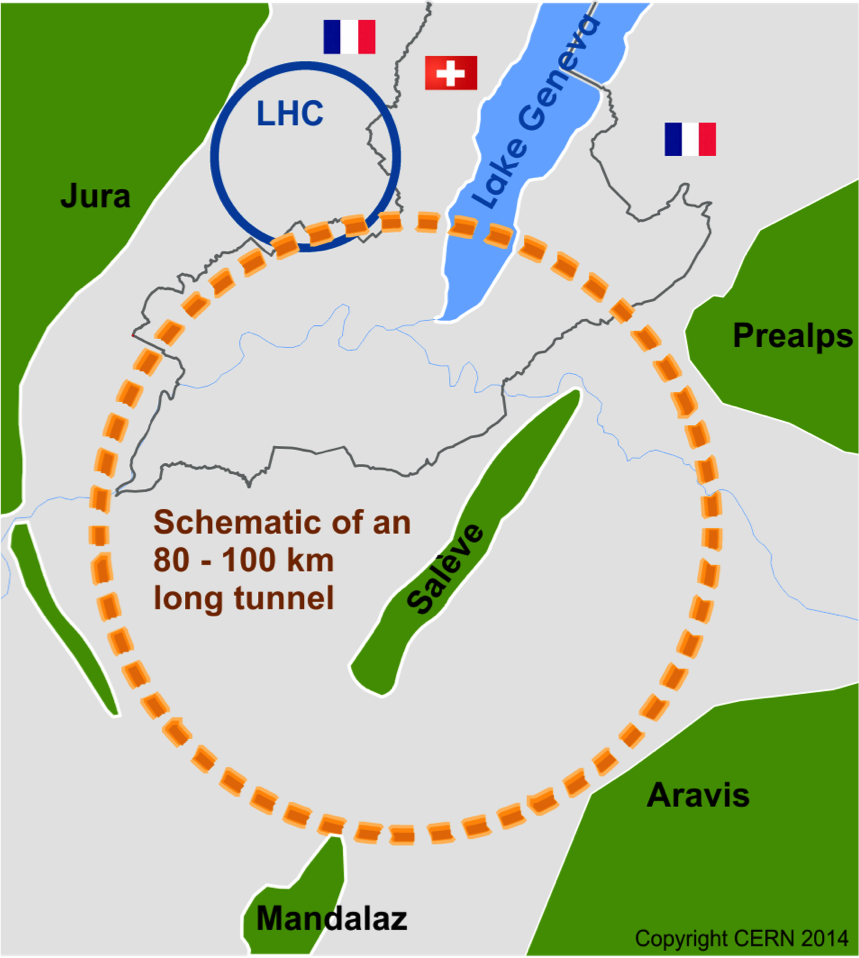
\includegraphics[width=\textwidth]{../figures/cernFCC}
	\end{columns}
	

\end{frame}

%%%%%%%%%%%%%%%%%%%%%%%%%%%%%
%         SLIDE             %
%%%%%%%%%%%%%%%%%%%%%%%%%%%%%
\begin{frame}
	\frametitle{2 FCCee detector concepts}
	
		\begin{itemize}
		\item The CLD detector concept (c.f. Oleksandr~Viazlo)
			\begin{itemize}
			\item An adaptation of the CLIC detector model 
			\\ $\Rightarrow$ (Silicon-based vertex and tracking detectors)
			\item Widely simulated with the ILCSoft
			\end{itemize}
		\item The IDEA detector concept (c.f. Franco Bedeschi)
			\begin{itemize}
			\item Simulated using FCCSW
			\end{itemize}
		\end{itemize}

	
	\begin{columns}
	\column{0.5\textwidth}
	
	\begin{block}{IDEA: Ultimate Goal}
	\begin{itemize}
	\item Vertex detector: MAPS
	\item Ultra-light drift chamber with PID (DCH)
	\item Double read-out calorimetry (DR)
        \item Additional disk layers to be placed in the space between DCH and DR 
	\item 2~T solenoidal magnetic field
	\item Instrumented return yoke
	\item Surrounded by large tracking volume (R$\sim$8~m) for very weakly coupled (long-lived) particles
	\end{itemize}
	\end{block}

	\column{0.5\textwidth}
        \vspace{-1cm}
	\centering
	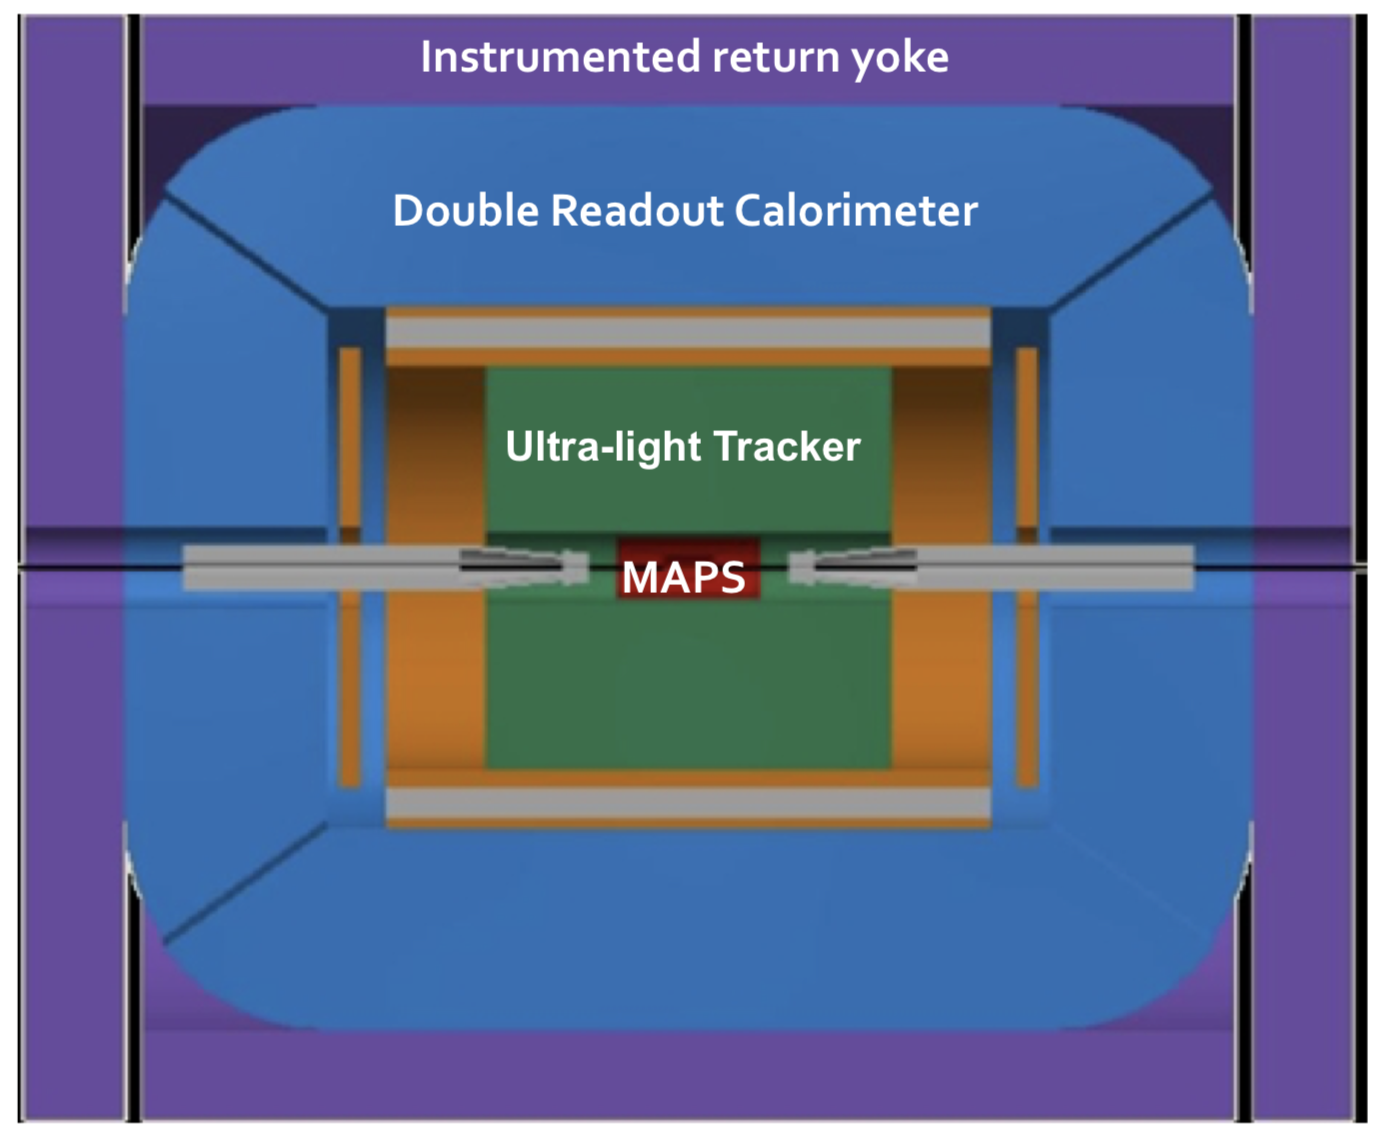
\includegraphics[width=\textwidth]{../figures/FCCeeIDEAConcept.png}
	\end{columns}

\end{frame}

%%%%%%%%%%%%%%%%%%%%%%%%%%%%%
%         SLIDE             %
%%%%%%%%%%%%%%%%%%%%%%%%%%%%%
\begin{frame}
	\frametitle{IDEA Drift Chamber (DCH)}
	
	\begin{columns}	
	\column{0.5\textwidth}
	
	\begin{itemize}
	\item \href{https://indico.cern.ch/event/656491/contributions/2939121/attachments/1629781/2597342/IDEA-CDCH_FCCweek18.pdf}{Talk by Giovanni Tassielli}
	\item Track reconstruction \& particle ID
	\end{itemize}


	\begin{block}{Parameters}
  	\begin{table}
    	\begin{adjustbox}{max width=\textwidth}
    	  \begin{tabular}{l l}
    	    \toprule
        % & Dimensions    \\
        % \hline
        Length & 4500 mm \\ 
        Inner radius & 345 mm \\
        Outer radius & 2000 mm\\
        Nb. layers & 112 \\
        Cell size & 12 mm to 14.7~mm\\
        Total nb. of sensitive wires & 56448 \\
        Total nb. of field wires & 282240 \\
        Total nb. of wires & 338688 \\
        Gas & GasHe\_90Isob\_10 \\
        Wire material & Aluminum \\
        Single cell resolution & 0.1 mm \\
        \bottomrule
      \end{tabular}
    	\end{adjustbox}
  	\end{table}
	\end{block}


	\column{0.5\textwidth}
	
	\begin{itemize}
	\item Field wires: provide a uniform electric field
	\item Sensitive wires: record signal
	\item Field to sensitive wire ratio: 5:1
	\end{itemize}
	
	
	\centering
	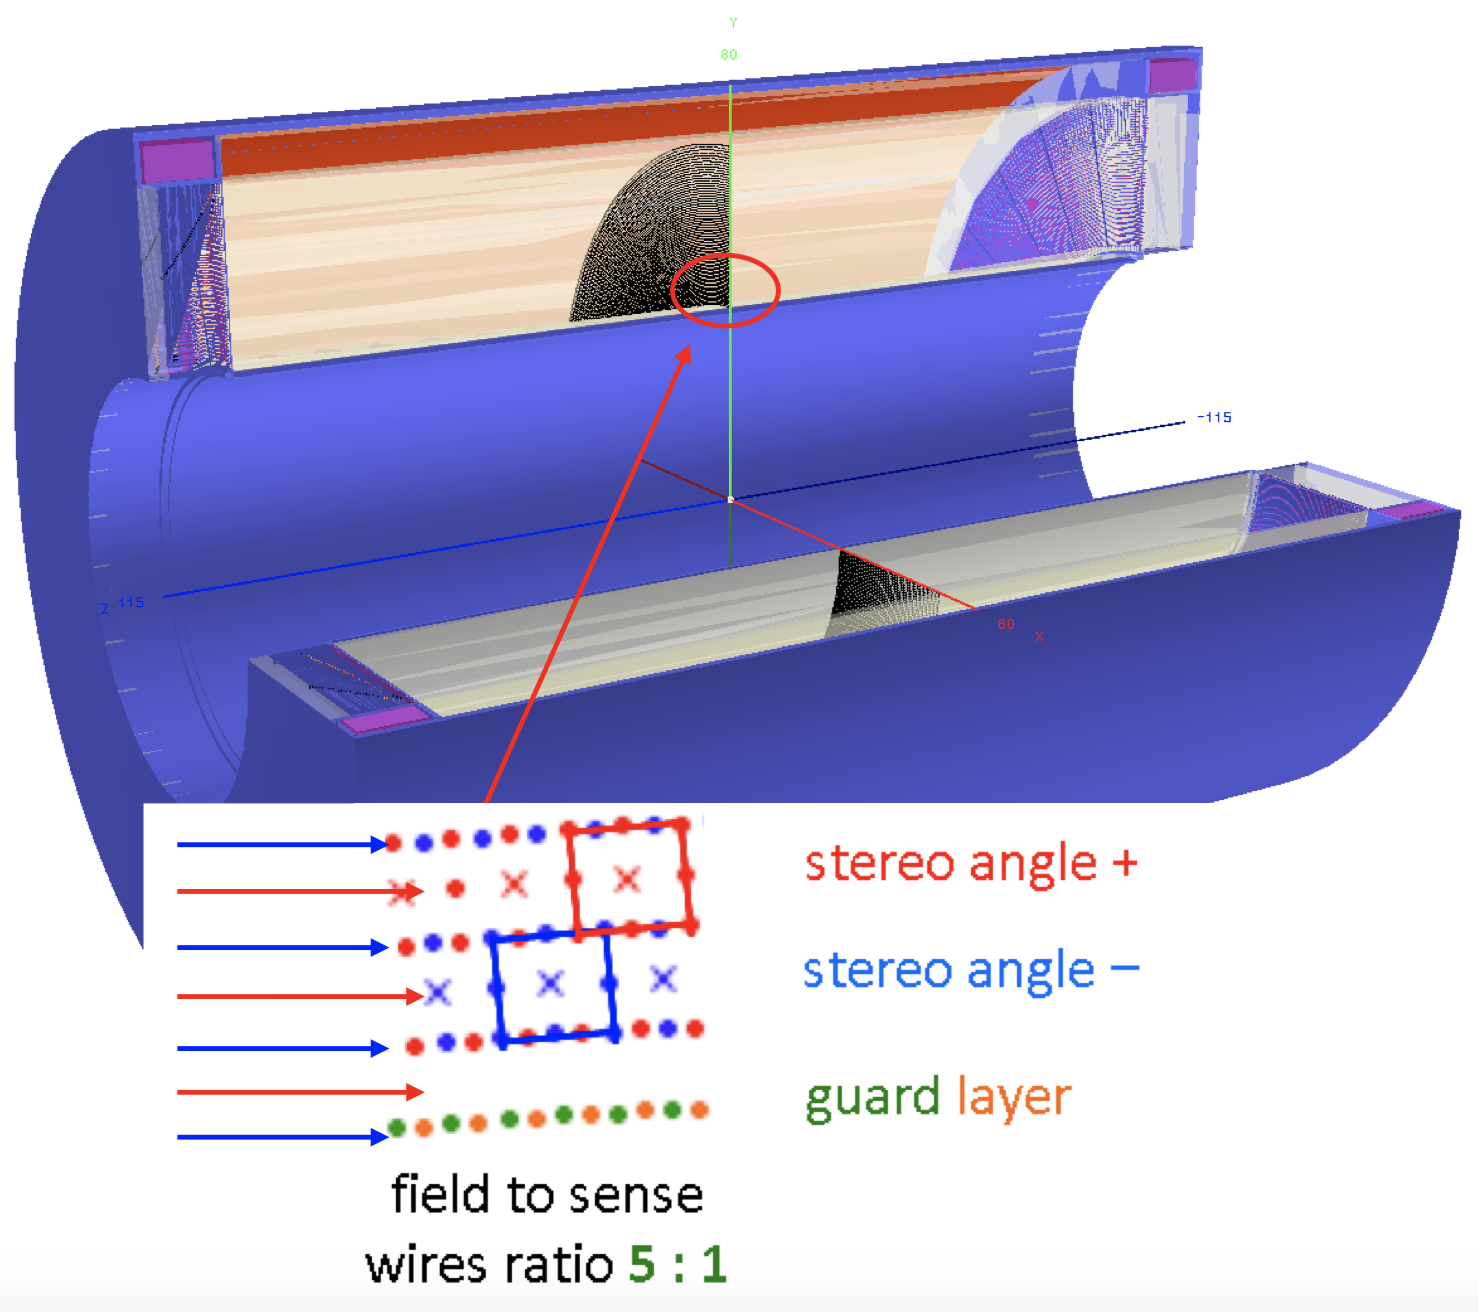
\includegraphics[width=\textwidth]{../figures/DriftChamber.png}
	\end{columns}
\end{frame}



%%%%%%%%%%%%%%%%%%%%%%%%%%%%%%
%%         SLIDE             %
%%%%%%%%%%%%%%%%%%%%%%%%%%%%%%
%\begin{frame}
%	\frametitle{FCCSW simulation chain}
%	
%	\begin{enumerate}
%	\item Detector geometry description with DD4hep
%		\begin{itemize}
%		\item Collaborative effort with CLIC, ILC and LHCb
%		\item The IR region and the VXD from CLD are as well implemented in DD4hep
%		\item Definition of the gas layers in the DCH 
%		\end{itemize}
%	\item Segmentation of the sensitive areas:
%		\begin{itemize}
%		\item Information on the position of the sense wires instead of placing physical volumes
%		\item Speed up the simulation
%		\end{itemize}
%	\item Geant4 simulation:
%		\begin{itemize}
%		\item Calculate the E\textsubscript{dep} for each ionisation action
%		\item Charge drift to the wires
%		\end{itemize}
%	\item Hit reconstruction:
%		\begin{itemize}
%		\item Combination of individual hit calculations from (3)
%		\item Calculation of the signal in the wire
%		\end{itemize}
%	\end{enumerate}		
%	
%        \centering
%	\smartdiagramset{back arrow disabled=true}
%  	\smartdiagram[flow diagram:horizontal]
%  	{%
%    	{Geometry\\DDhep}, Segmentation, {Geant4 \\simulation}, Hit Reconstruction%
%  	}
%
%\end{frame}

%%%%%%%%%%%%%%%%%%%%%%%%%%%%%
%         SLIDE             %
%%%%%%%%%%%%%%%%%%%%%%%%%%%%%
\begin{frame}
	\frametitle{FCCSW simulation chain}
	
    \centering
	\smartdiagramset{back arrow disabled=true}
	\usebeamercolor{background canvas}
  	\smartdiagram[flow diagram:horizontal]
  	{%
    	{Geometry\\DDhep}, Segmentation, {Geant4 \\simulation}, Hit Reconstruction%
  	}


\end{frame}

%%%%%%%%%%%%%%%%%%%%%%%%%%%%%
%         SLIDE             %
%%%%%%%%%%%%%%%%%%%%%%%%%%%%%
\begin{frame}
	\frametitle{FCCSW simulation chain}
	
    \centering
	\smartdiagramset{back arrow disabled=true}
	\usebeamercolor{background canvas}
  	\smartdiagram[flow diagram:horizontal]
  	{%
    	{Geometry\\DDhep}, Segmentation, {Geant4 \\simulation}, Hit Reconstruction%
  	}

	\vspace{1cm}
	\centering
	\Huge{1. Geometry description}
\end{frame}


%%%%%%%%%%%%%%%%%%%%%%%%%%%%%
%         SLIDE             %
%%%%%%%%%%%%%%%%%%%%%%%%%%%%%
\begin{frame}
	\frametitle{1. Geometry description}
	
	\begin{itemize}
	\item Same interaction region (beampipe \& instrumentation, VXD) as the CLD concept
	\item New implementation: drift chamber $\Rightarrow$ only the gas volume is placed
	\end{itemize}
	
	\begin{block}{Visualisation with FCCSW}
	\centering
	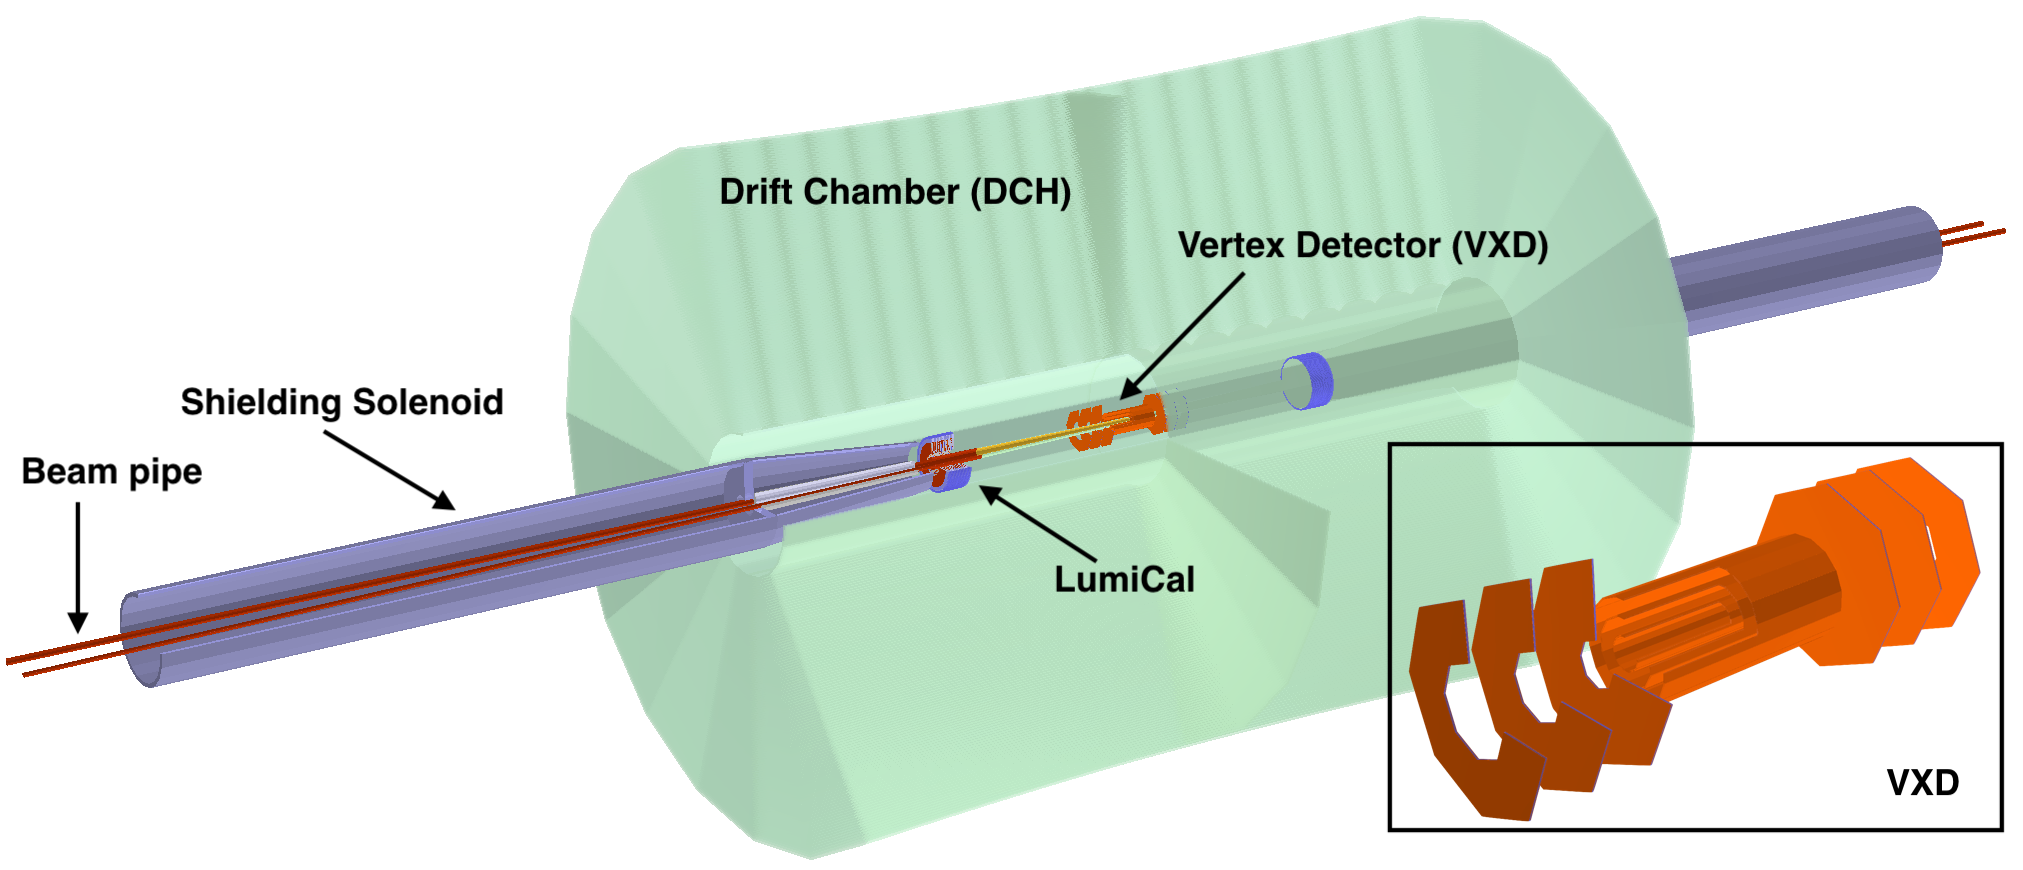
\includegraphics[width=\textwidth]{../figures/FCCeeIDEA_IR_description_zoomVXD.png}
	\end{block}

\end{frame}


%%%%%%%%%%%%%%%%%%%%%%%%%%%%%
%         SLIDE             %
%%%%%%%%%%%%%%%%%%%%%%%%%%%%%
\begin{frame}
	\frametitle{FCCSW simulation chain}
	
    \centering
	\smartdiagramset{back arrow disabled=true}
	\usebeamercolor{background canvas}
  	\smartdiagram[flow diagram:horizontal]
  	{%
    	{Geometry\\DDhep}, Segmentation, {Geant4 \\simulation}, Hit Reconstruction%
  	}

	\vspace{1cm}
	\centering
	\Huge{2. Segmentation}
	
\end{frame}
%%%%%%%%%%%%%%%%%%%%%%%%%%%%%
%         SLIDE             %
%%%%%%%%%%%%%%%%%%%%%%%%%%%%%

\begin{frame}
  \frametitle{2. Segmentation Strategy for DCH (1)}

	\vspace{1cm}
	
	\begin{columns}[t]
	\column{0.5\textwidth}
	\begin{itemize}
    \item Large number of wires $\Rightarrow$ fast way to find the
      location of the closest wire hit
    \item Projection of the hit positions into the x-y plane
    \item Consider the z axis to compensate for the stereo angle of the wires
    \end{itemize}
    
    \column{0.5\textwidth}
	\centering
	\begin{itemize}
	\item Example: MEG II DCH
	\end{itemize}
	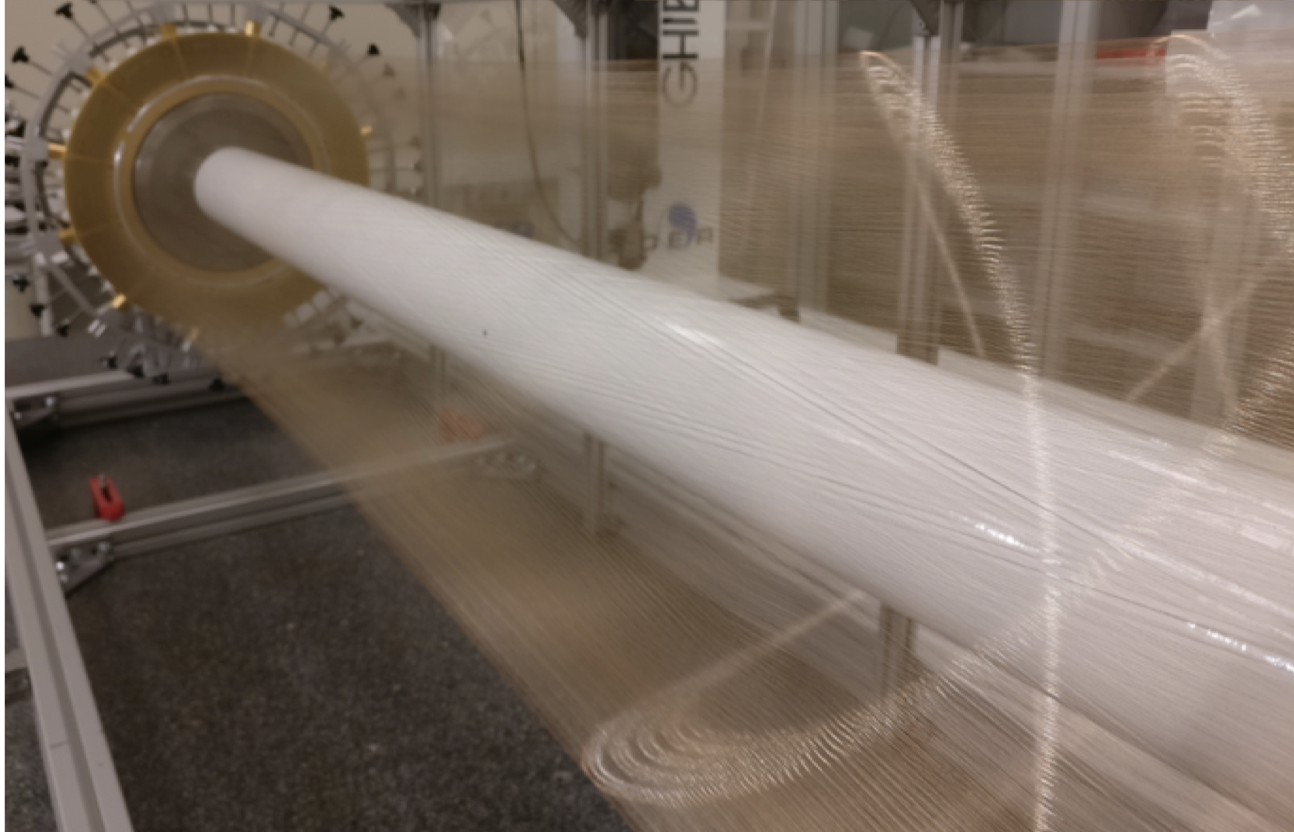
\includegraphics[width=0.7\textwidth]{../figures/MEGDCH.png}
    \end{columns}
	
	\vspace{-0.5cm}
    \begin{columns}
      \column{0.33\textwidth}
      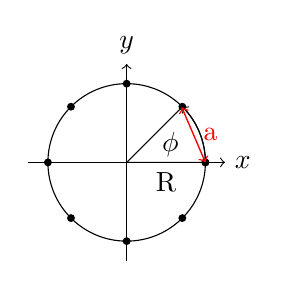
\begin{tikzpicture}[scale=0.5]

        \pgfmathsetmacro{\R}{2}
        \pgfmathsetmacro{\wireAng}{45}
        
        \coordinate (O) at (0,0);
        \foreach \angle in 
        {0,45,...,360} 
        { 
          \fill (\angle:\R) circle (0.1cm); 
        } 
        \draw (0,0) circle (\R);

        \draw 
        (\R,0) coordinate (xcoord) -- 
        node[midway,below] {R} (O) -- 
        (\wireAng:\R) coordinate (slcoord)
        pic [draw,->,angle radius=1cm,"$\phi$"] {angle = xcoord--O--slcoord};

        \draw[<->,line width=0.5pt,red] (\R, 0) -- (1.4, 1.4) node
        (deltay) [midway,right] {a};

        \begin{scope}[]
          \draw[->] (-2.5,0) -- (2.5,0) node[right] {$x$};
          \draw[->] (0,-2.5) -- (0,2.5) node[above] {$y$};
        \end{scope}
      \end{tikzpicture}

      \column{0.33\textwidth}
    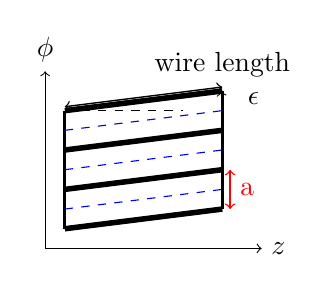
\begin{tikzpicture}[scale=0.5]
      \begin{scope}
        \coordinate (origin) at (0,4);

        \draw[->] (-0.5,0.5) -- (5,0.5) node[right] {$z$};
        \draw[->] (-0.5, 0.5) -- (-0.5,5) node[above] {$\phi$};

        \draw[-,line width=1pt] (0, 1) -- (0, 4);
        \draw[-,line width=1pt] (4, 1.5) -- (4, 4.5);

        \draw[-,line width=2pt] (0, 1) -- (4, 1.5);
        \draw[-,line width=2pt] (0, 2) -- (4, 2.5);
        \draw[-,line width=2pt] (0, 3) -- (4, 3.5);
        \draw[-,line width=2pt] (0, 4) -- (4, 4.5) node
        (pivot) [] {};
        \draw[<->,line width=0.5pt] (0, 4.1) -- (4, 4.6) node
        (length) [above] {wire length};
        \draw[<->,line width=0.5pt,red] (4.2, 1.5) -- (4.2, 2.5) node
        (deltay) [midway, right] {a};

        \draw[-,dashed, line width=0.5pt] (origin) -- (3, 4) node
        (horizon) [] {};
        \pic [draw, ->, "$\epsilon$", angle eccentricity=1.2, angle radius=2cm] {angle = horizon--origin--pivot};


        \draw[-,dashed, blue] (0, 1.5) -- (4, 2);
        \draw[-, dashed, blue] (0, 2.5) -- (4, 3);
        \draw[-, dashed, blue] (0, 3.5) -- (4, 4);

        % \draw[-,blue,line width=1pt] (2, 5) -- (2, 0.7) node
        % (segz) [right] {z segmentation (w)};
      \end{scope}
    \end{tikzpicture}

    \column{0.33\textwidth}

    \end{columns}


\end{frame}

%%%%%%%%%%%%%%%%%%%%%%%%%%%%%
%         SLIDE             %
%%%%%%%%%%%%%%%%%%%%%%%%%%%%%
\begin{frame}
	\frametitle{2. Segmentation: validation in simulation (2)}
		
	\begin{columns}[t]
		\column{0.5\textwidth}
		\begin{itemize}
		\item Information on the location of the sensitive wires \vspace{0.2cm}
		\item Associates a unique wire ID (cellID) to the wires \vspace{0.2cm}
		\item Different granularity for different layers in the DCH \vspace{0.2cm}
		\item The segmentation information is created while building geometry \vspace{0.2cm} \\
			$\Rightarrow$ Accessible in every step of the simulation
		\end{itemize}
	
		\column{0.5\textwidth}	
		\begin{itemize}
		\item First layer of the DCH
		\item Hits having the same wire ID are shown by the same color
		\item Validates the segmentation
		\end{itemize}
		\centering
		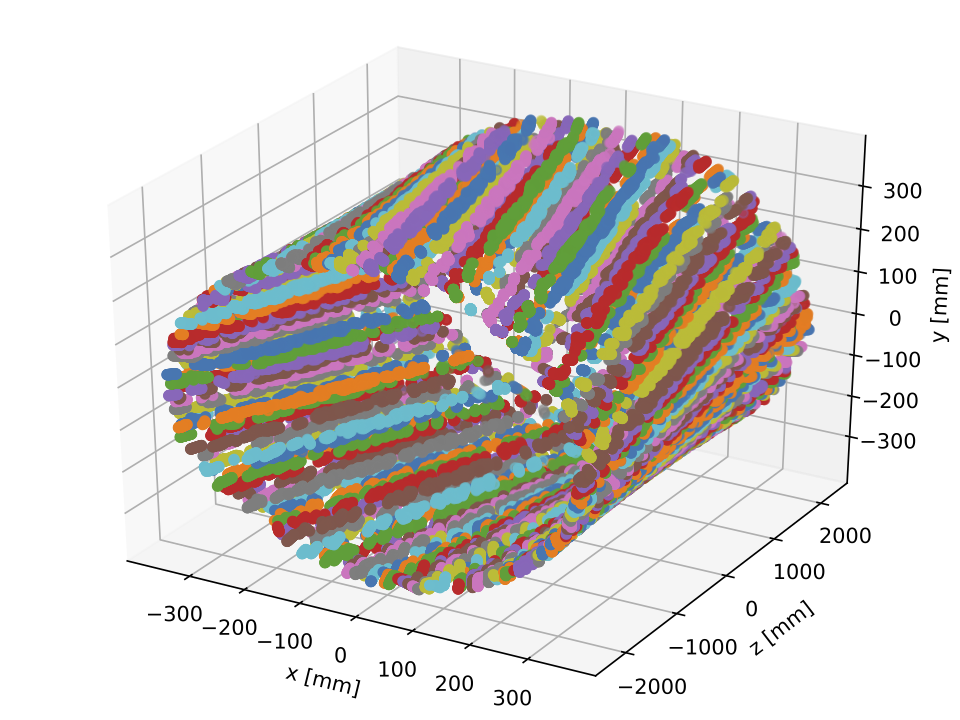
\includegraphics[width=\textwidth]{../figures/allHits}
	\end{columns}
	
\end{frame}

%%%%%%%%%%%%%%%%%%%%%%%%%%%%%
%         SLIDE             %
%%%%%%%%%%%%%%%%%%%%%%%%%%%%%
\begin{frame}
	\frametitle{FCCSW simulation chain}
	
    \centering
	\smartdiagramset{back arrow disabled=true}
	\usebeamercolor{background canvas}
  	\smartdiagram[flow diagram:horizontal]
  	{%
    	{Geometry\\DDhep}, Segmentation, {Geant4 \\simulation}, Hit Reconstruction%
  	}

	\vspace{1cm}
	\centering
	\Huge{3. Geant4 hit simulation \& reconstruction}
	
\end{frame}

%%%%%%%%%%%%%%%%%%%%%%%%%%%%%
%         SLIDE             %
%%%%%%%%%%%%%%%%%%%%%%%%%%%%%
\begin{frame}
	\frametitle{3. Hit simulation and reconstruction of the DCH}

	\begin{block}{Hit Simulation}
	\begin{itemize}
	\item Geant4: Stepping in the gas with a G4Step length of 2~mm 
	\item Reject ionisation acts with:
		\begin{itemize}
		\item E\textsubscript{dep}$<$~10~eV
		\item \texttt{G4Step} length~$<~5\mu$m
		\end{itemize} 
	
	\item Drift the charge deposition to the nearest wire 
		\begin{itemize}
		\item Compute the distance of the closest approach
		\item Calculate the drift time assuming a constant drift velocity of 2~cm/$\mu$s
		\item Calculate the total time of the hit \\
		\begin{equation}
	      t_{hit} = t_{drift}+t_{\text{signal}}+t_{\text{particle flight}}
    		\end{equation}
		\end{itemize} 
	\end{itemize}
	\end{block}
		
	\begin{block}{Reconstruction}
		\begin{itemize}
		\item \textcolor{Red}{Hit}: regroup the E\textsubscript{dep} with a drift time smaller than the maximum drift time in the cell
		\end{itemize}
	\end{block}

	
	
	
\end{frame}


%%%%%%%%%%%%%%%%%%%%%%%%%%%%%
%         SLIDE             %
%%%%%%%%%%%%%%%%%%%%%%%%%%%%%
\begin{frame}
	\frametitle{Coverage of the vertex detector \& the drift chamber}
	
	\begin{itemize}
		\item Number of layers hit by 100~GeV $\mu-$ 
		\begin{itemize}

		\item $\theta=0^{\circ}$: in the forward direction
		\item $\theta=90^{\circ}$: in the barrel
		\item Averaged over $\phi$	
		\end{itemize}
	\end{itemize}
		
	\begin{columns}	
		\column{0.5\textwidth}	
		\begin{block}{VXD}
		\centering
		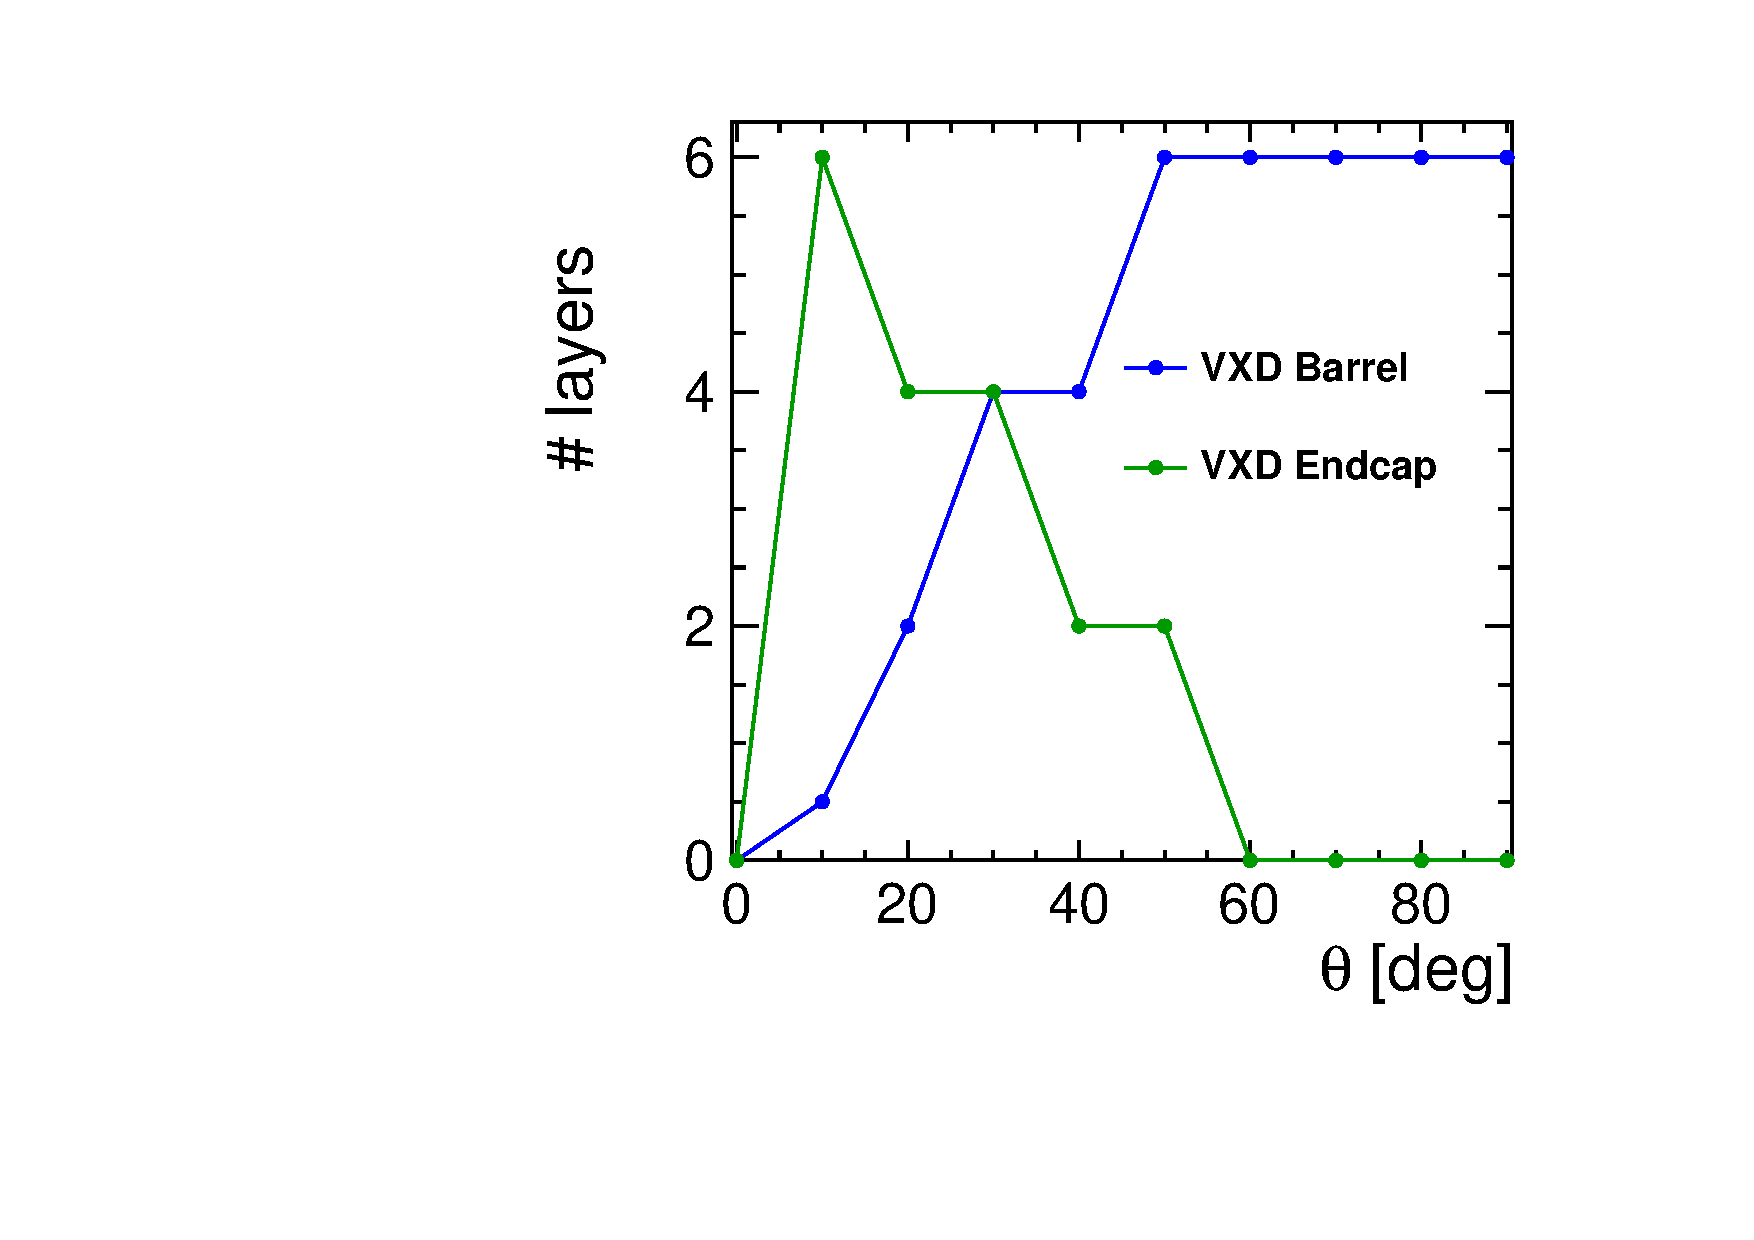
\includegraphics[width=\textwidth]{../figures/theta_nbHits_VXD.pdf}
		\end{block}
	
		\column{0.5\textwidth}	
		\begin{block}{DCH}
		\centering
		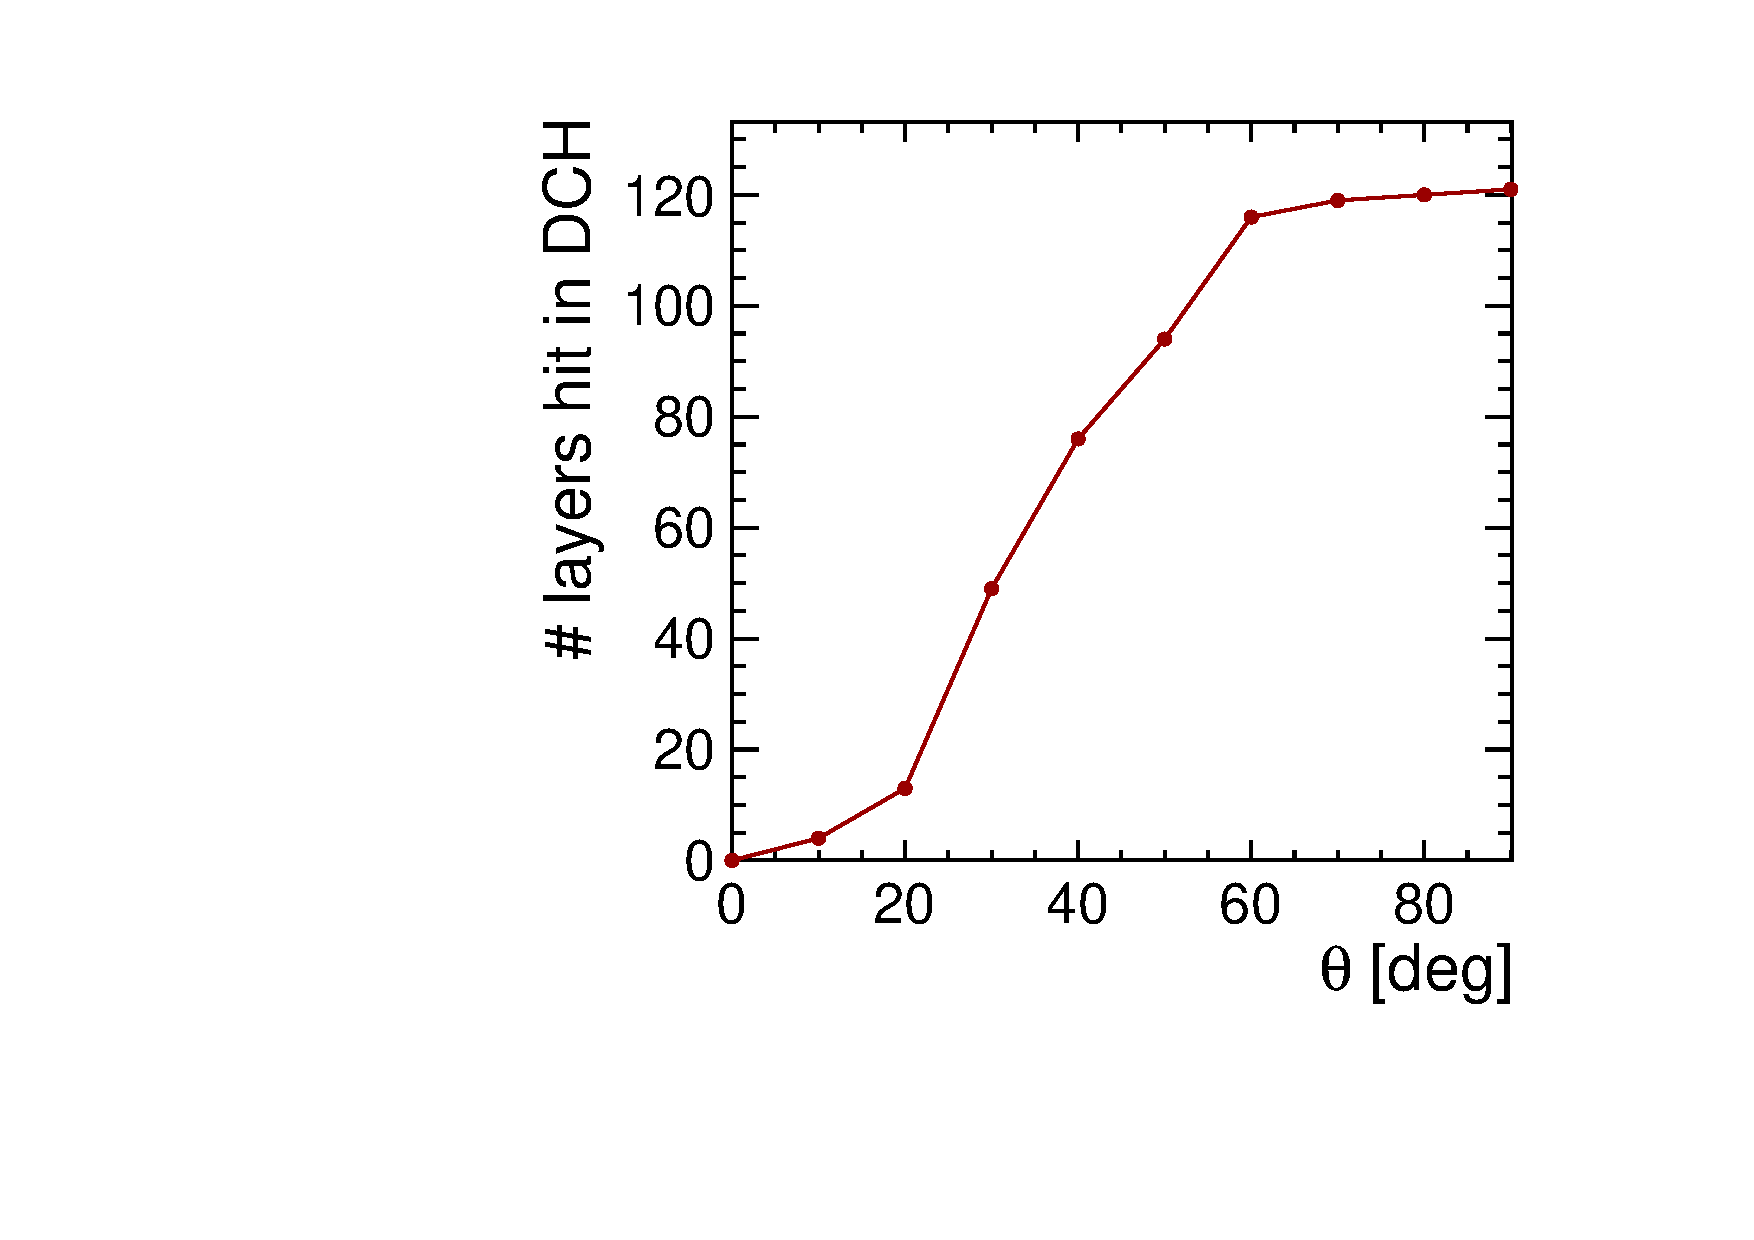
\includegraphics[width=\textwidth]{../figures/theta_nbHits_DCH.pdf} 	
		\end{block}
	\end{columns}
	
	
\end{frame}


%%%%%%%%%%%%%%%%%%%%%%%%%%%%%
%         SLIDE             %
%%%%%%%%%%%%%%%%%%%%%%%%%%%%%
\begin{frame}
	\frametitle{Impact of the beam background on the interaction region (IR)}

	\begin{columns}
	\column{0.4\textwidth}
	\begin{itemize}
	\item The effect of $e^{+}e^{-}$ pairs from $\gamma\gamma$ collisions (dominated by beamstrahlung photons)
	\item Pairs generated using the GuineaPig software (c.f. Georgios Voutsinas)
	\item E\textsubscript{cm} = 365~GeV
	\item Total nb. of particles: $\sim6200$ / BX
        \item A fortiori, no tracks reach the DCH wires\vspace{0.2cm}
	\end{itemize}		
	\column{0.6\textwidth}
		\centering
		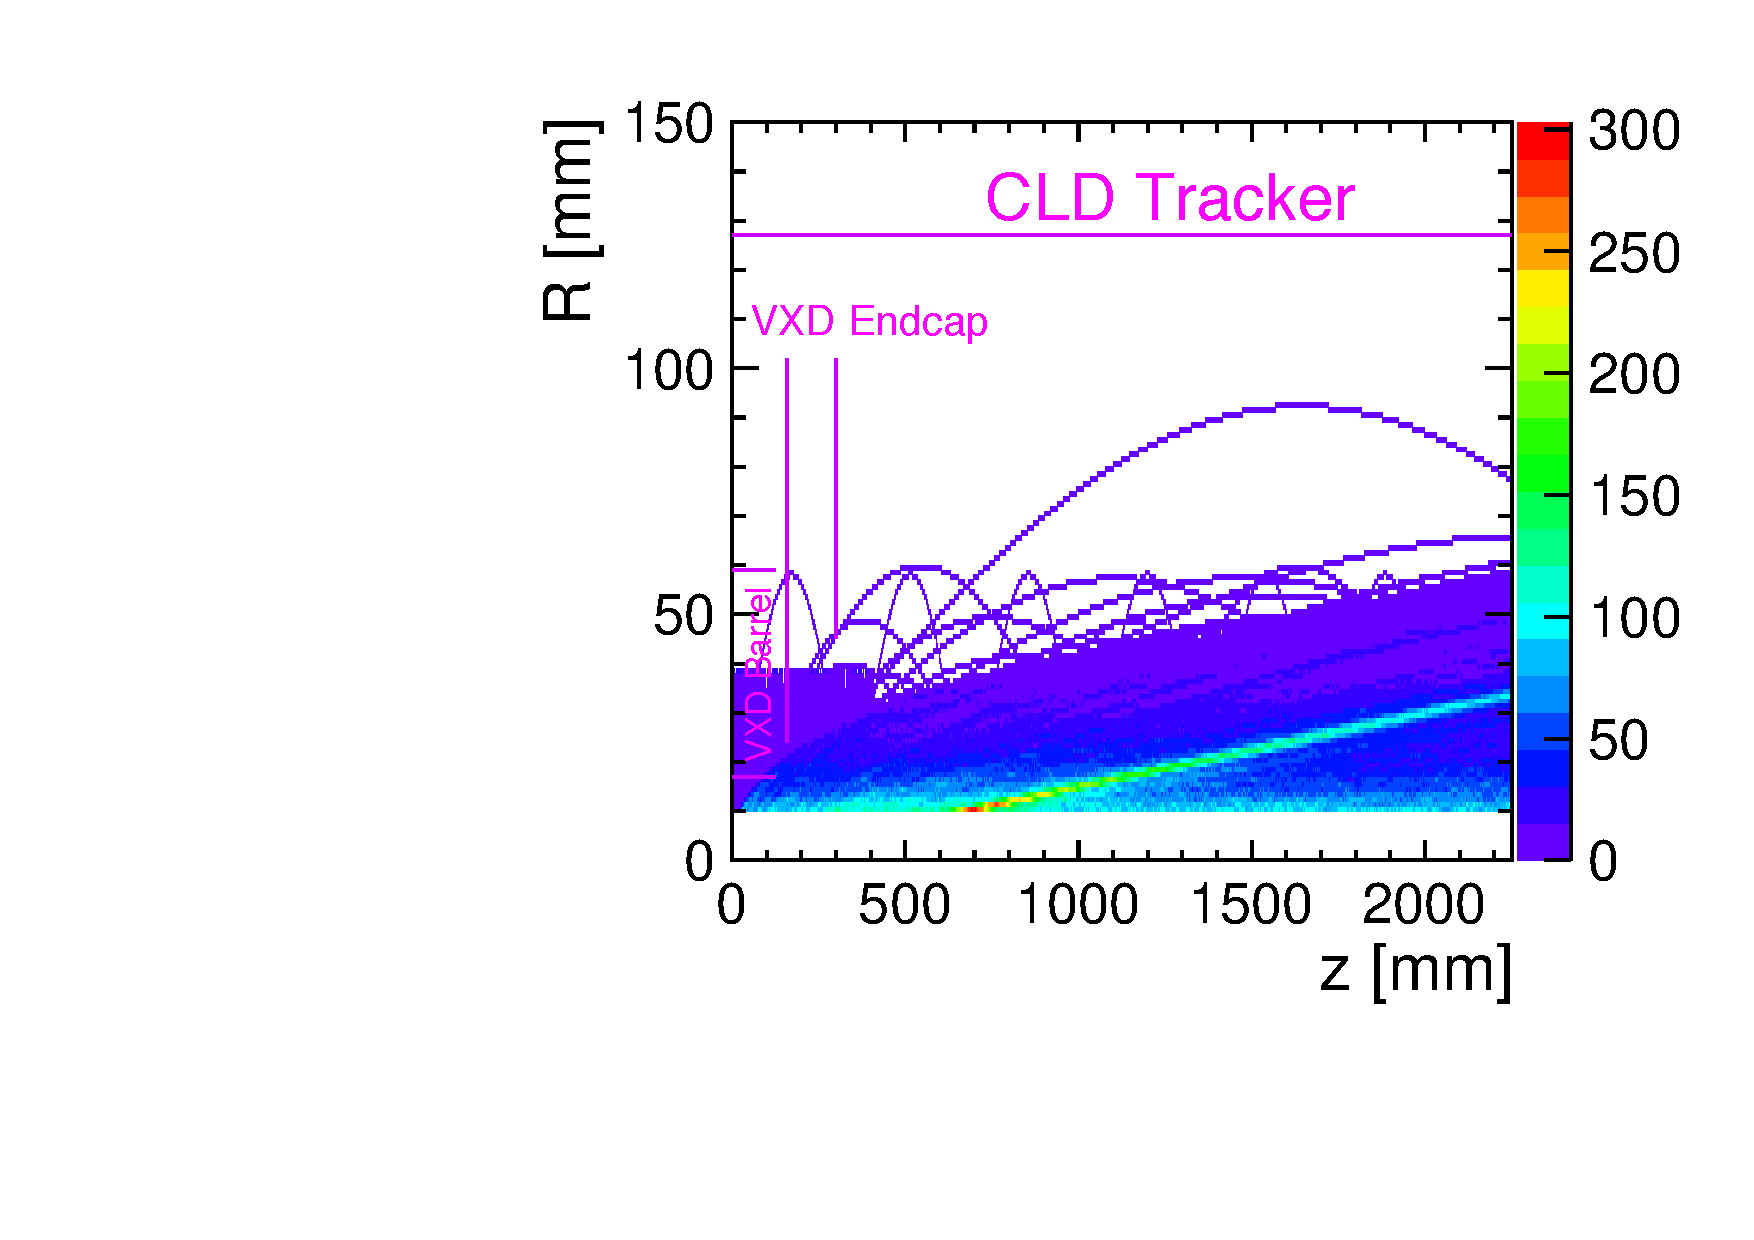
\includegraphics[width=\textwidth]{../figures/pairs_R_Z_legend.pdf}
	\end{columns}	
	
\end{frame}

%%%%%%%%%%%%%%%%%%%%%%%%%%%%%
%         SLIDE             %
%%%%%%%%%%%%%%%%%%%%%%%%%%%%%
\begin{frame}
	\frametitle{Impact of incoherent pairs in the VXD}

	\begin{itemize}
	\item The number of hits is averaged over 30 BX
	\end{itemize}	
	
	
	\begin{columns}
	\column{0.5\textwidth}
		\begin{itemize}
		\item Vertex Barrel
		\end{itemize}
		\centering
		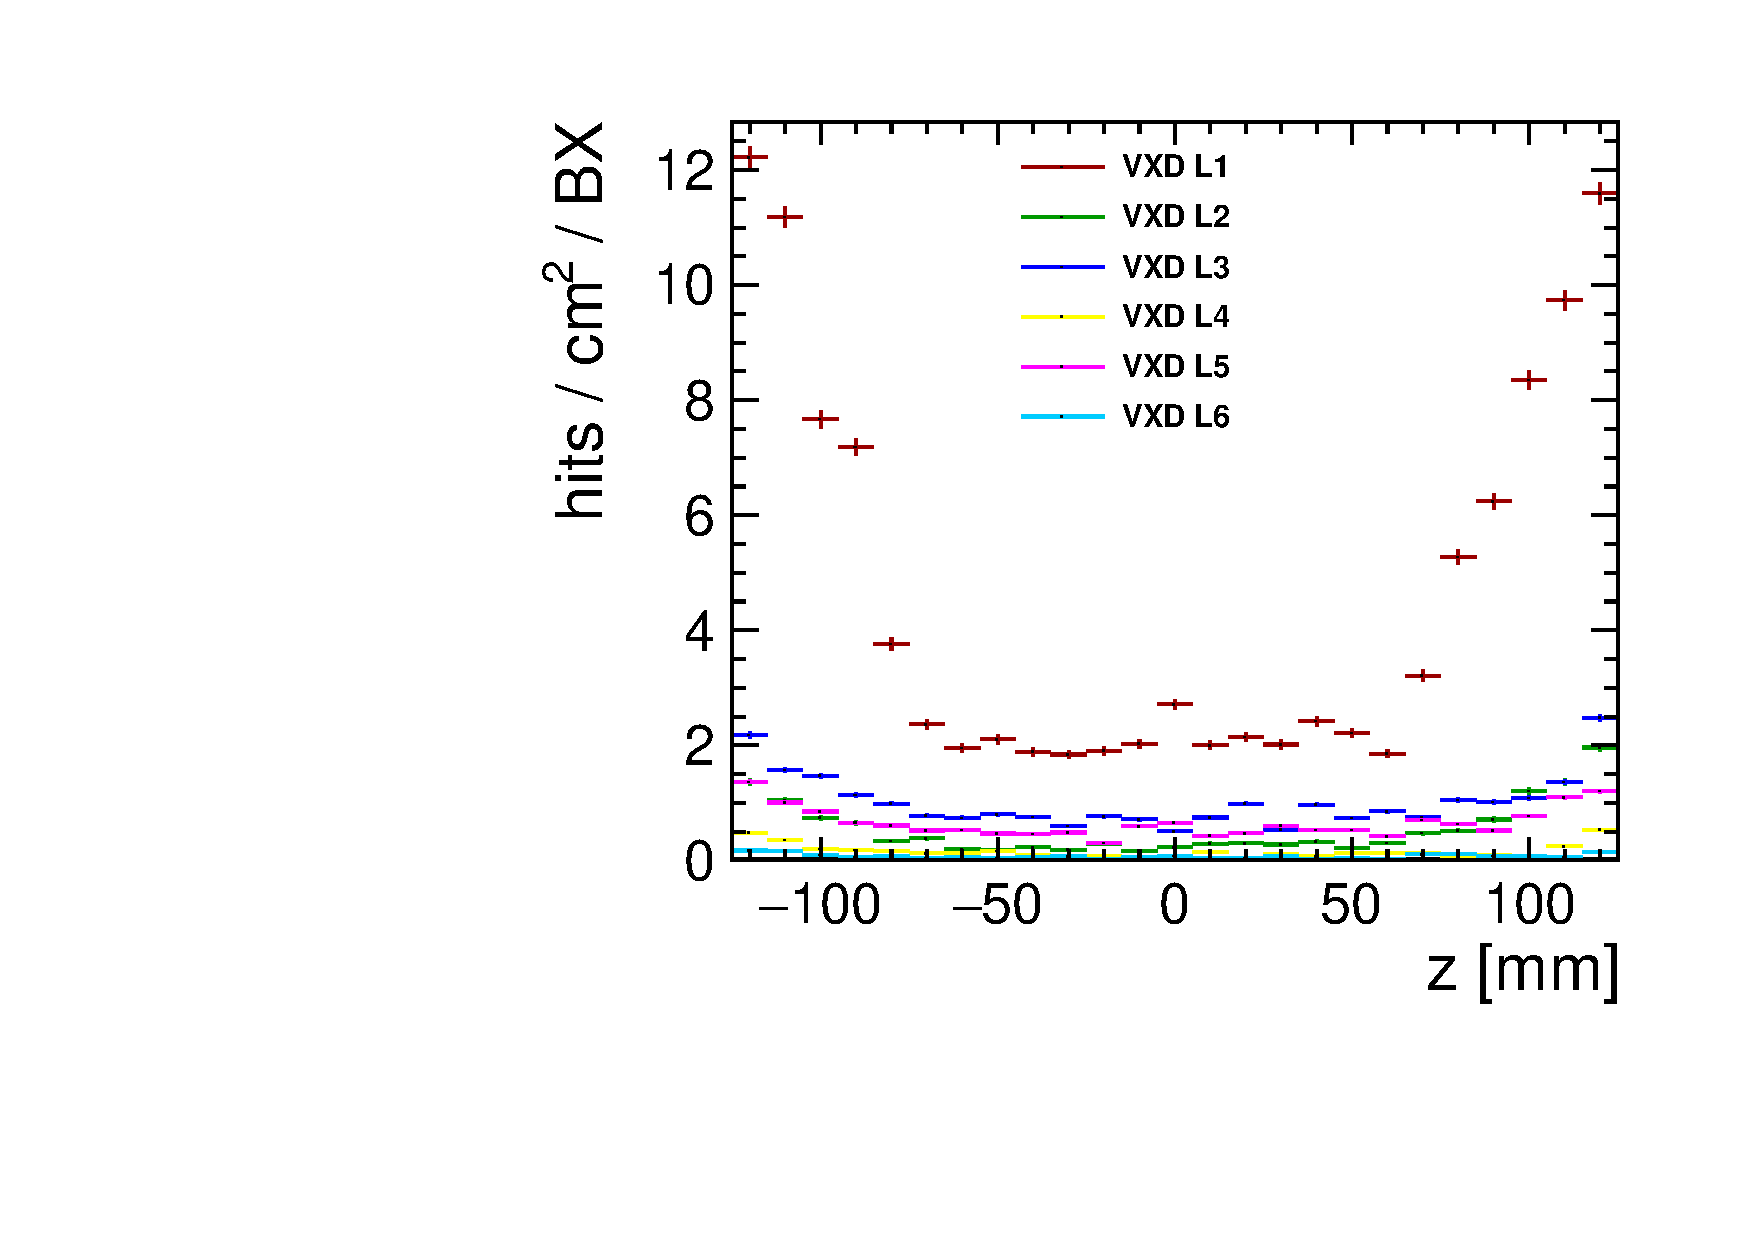
\includegraphics[width=\textwidth]{../figures/occupancy_VXD_barrel.pdf}
		
	\column{0.5\textwidth}
		\begin{itemize}
		\item Vertex Endcap
		\end{itemize}
		\centering
		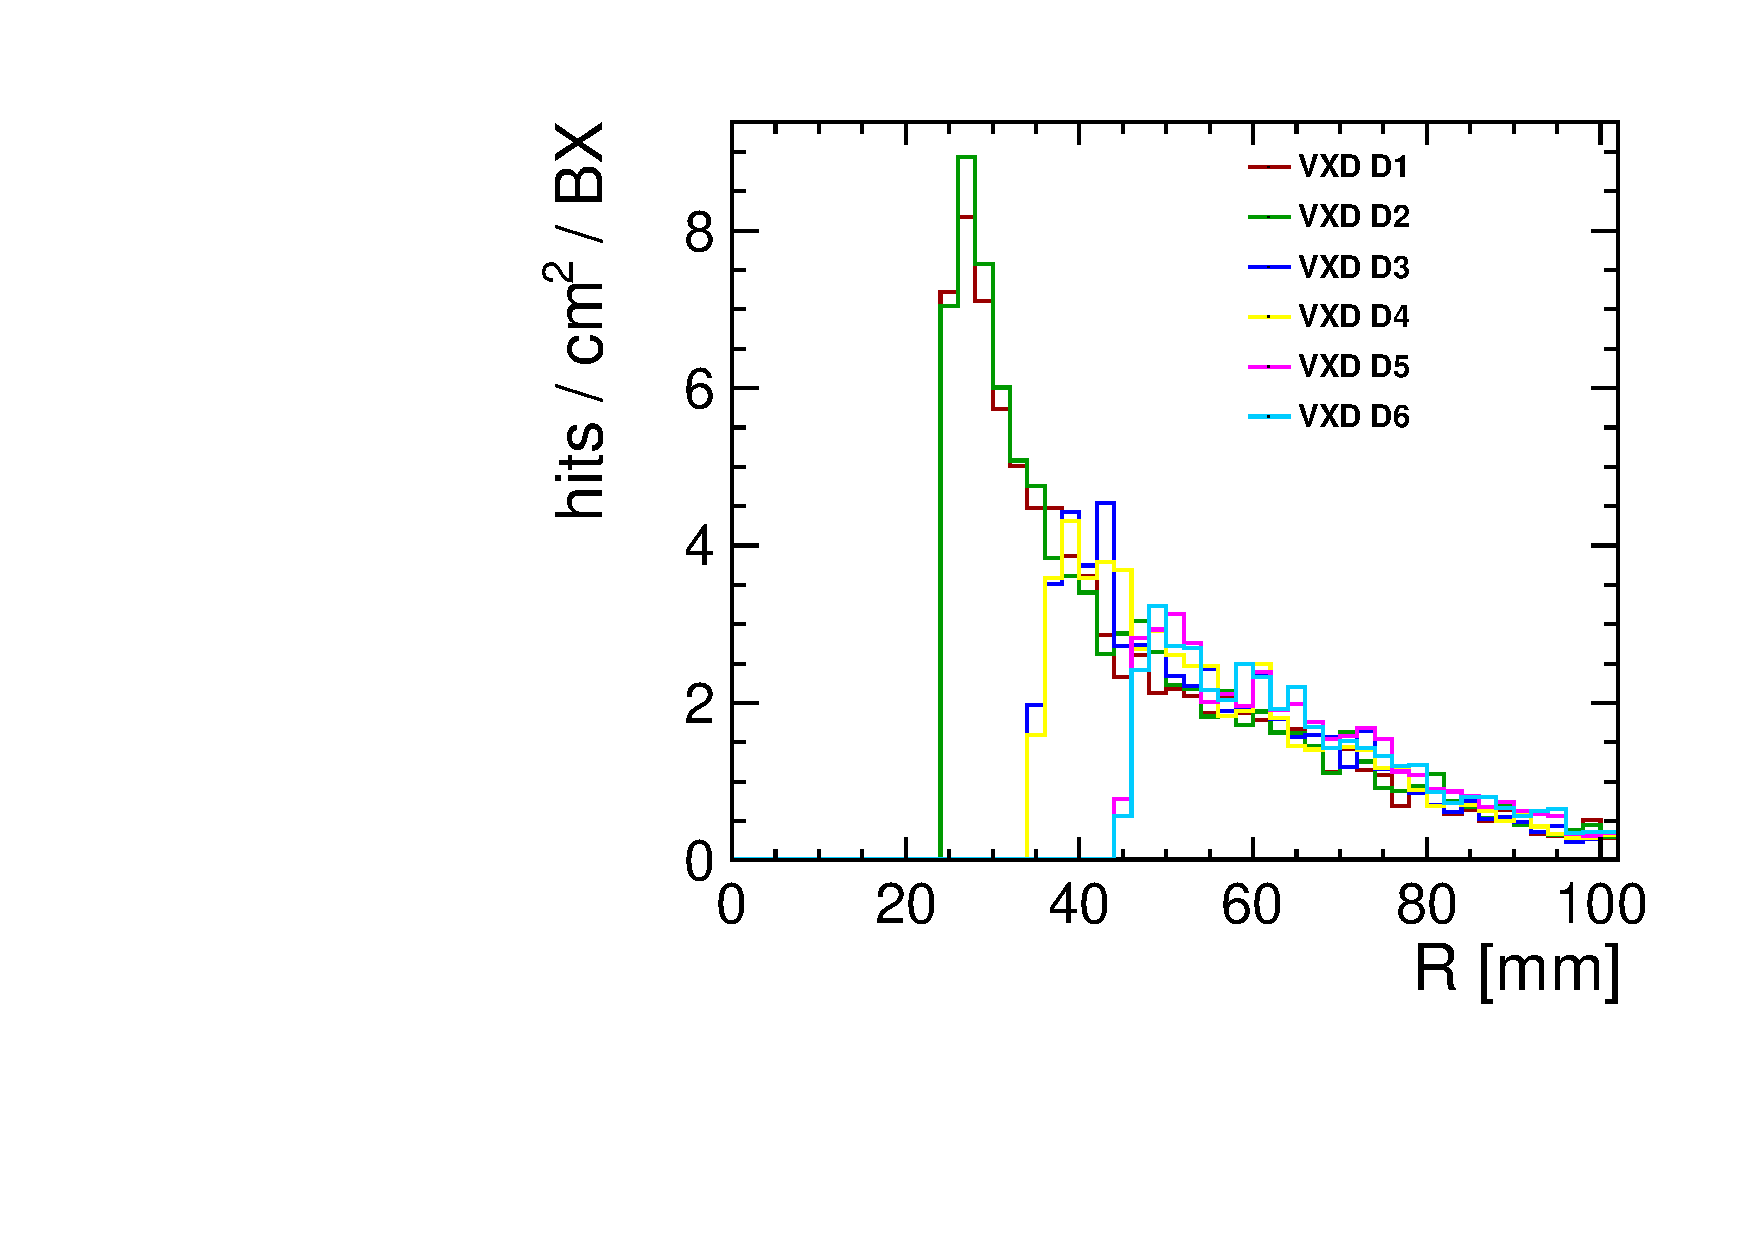
\includegraphics[width=\textwidth]{../figures/occupancy_VXD_endcap.pdf}
	\end{columns}
	
	\begin{itemize}
	\item Comparisons with the ILCSoft in progress \& encouraging
	\item The level of this background does not pose problem for pattern recognition
	\end{itemize}	
	
\end{frame}


%%%%%%%%%%%%%%%%%%%%%%%%%%%%%
%         SLIDE             %
%%%%%%%%%%%%%%%%%%%%%%%%%%%%%
\begin{frame}
	\frametitle{Impact of incoherent pairs in the DCH: work in progress}

	\begin{columns}[t]
	\column{0.5\textwidth}
		\begin{itemize}
		\item Most of the hits in the DCH are due to the backscattering   \vspace{0.2cm}
		\item Current simulations show a background level of $\sim3.5\%$ \vspace{0.2cm}
		\item Expected acceptable level of occupancy for a successful pattern recognition: $\sim5\%$ \vspace{0.2cm}

		\item The current estimation of the occupancy is pessimistic due to unclear behaviour of \textsc{Geant4} at the boundary conditions and the lack of calorimeter, magnet and yoke around the DCH in the simulation \\ \vspace{1cm}
		\textbf{\textcolor{Green}{$\Rightarrow$ Work in progress - stay tuned!}}
		\end{itemize}	
	
	\column{0.5\textwidth}
	
	\begin{itemize}
	\item Vertices of backscattering particles
	\end{itemize}
	\centering

    \begin{tikzpicture}
      \node[anchor=south west,inner sep=0] (image) at
      (0,0){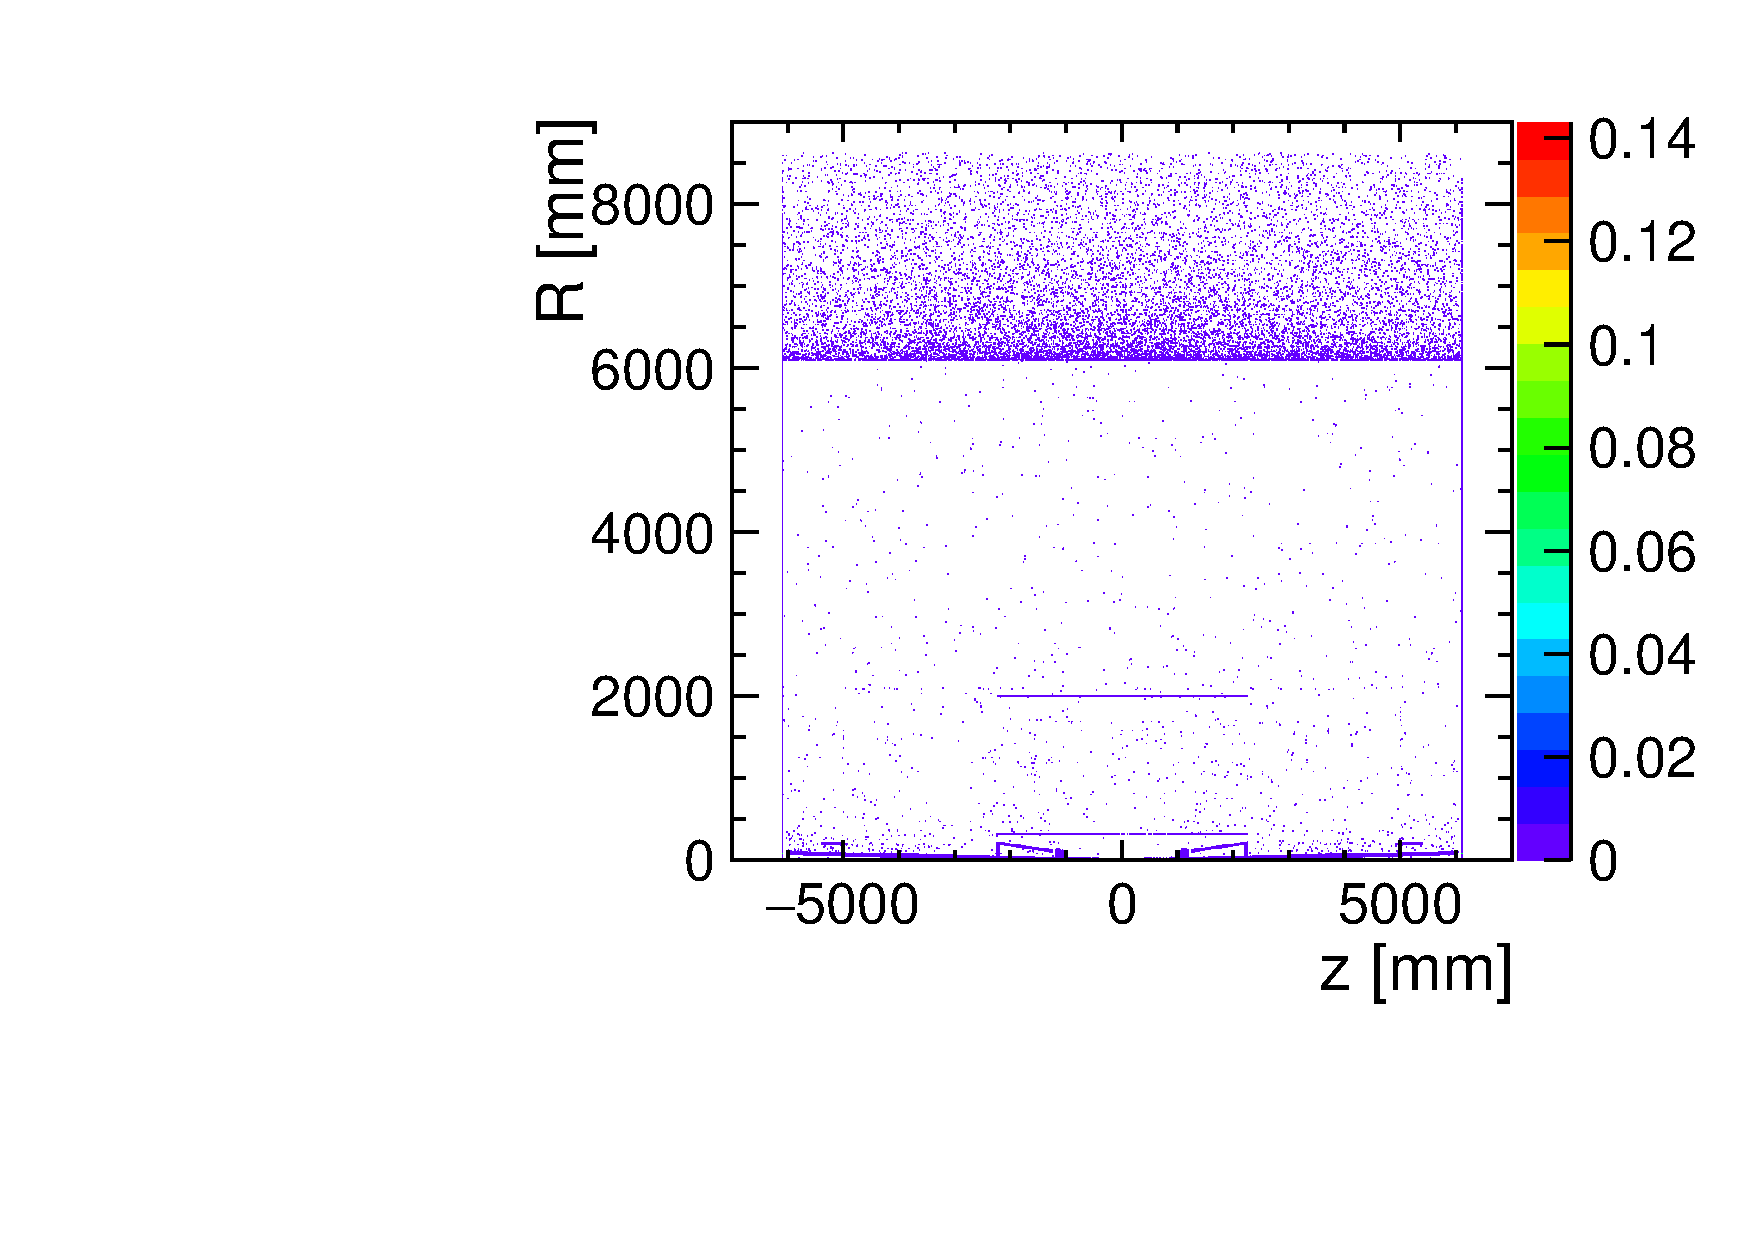
\includegraphics[width=\textwidth]{../figures/secondaryVertices.pdf}};
      \begin{scope}[x={(image.south east)},y={(image.north west)}]

%      \draw[help lines,xstep=.1,ystep=.1] (0, 0) grid (1,1);
%         \foreach \x in {0,1,...,9} { \node [anchor=north] at (\x/10,0) {0.\x}; }
%         \foreach \y in {0,1,...,9} { \node [anchor=east] at (0,\y/10)
%         {0.\y}; }
%        
		\node[above] at (0.5, 0.95) {Boundaries of the simulation}; 
		\draw[->, very thick](0.5, 0.95) -- (0.5, 0.8);      
		\draw[->, very thick](0.4, 0.95) -- (0.22, 0.5); 
		\draw[->, very thick](0.6, 0.95) -- (0.78, 0.5); 
        
      \end{scope}
    \end{tikzpicture}
	
	%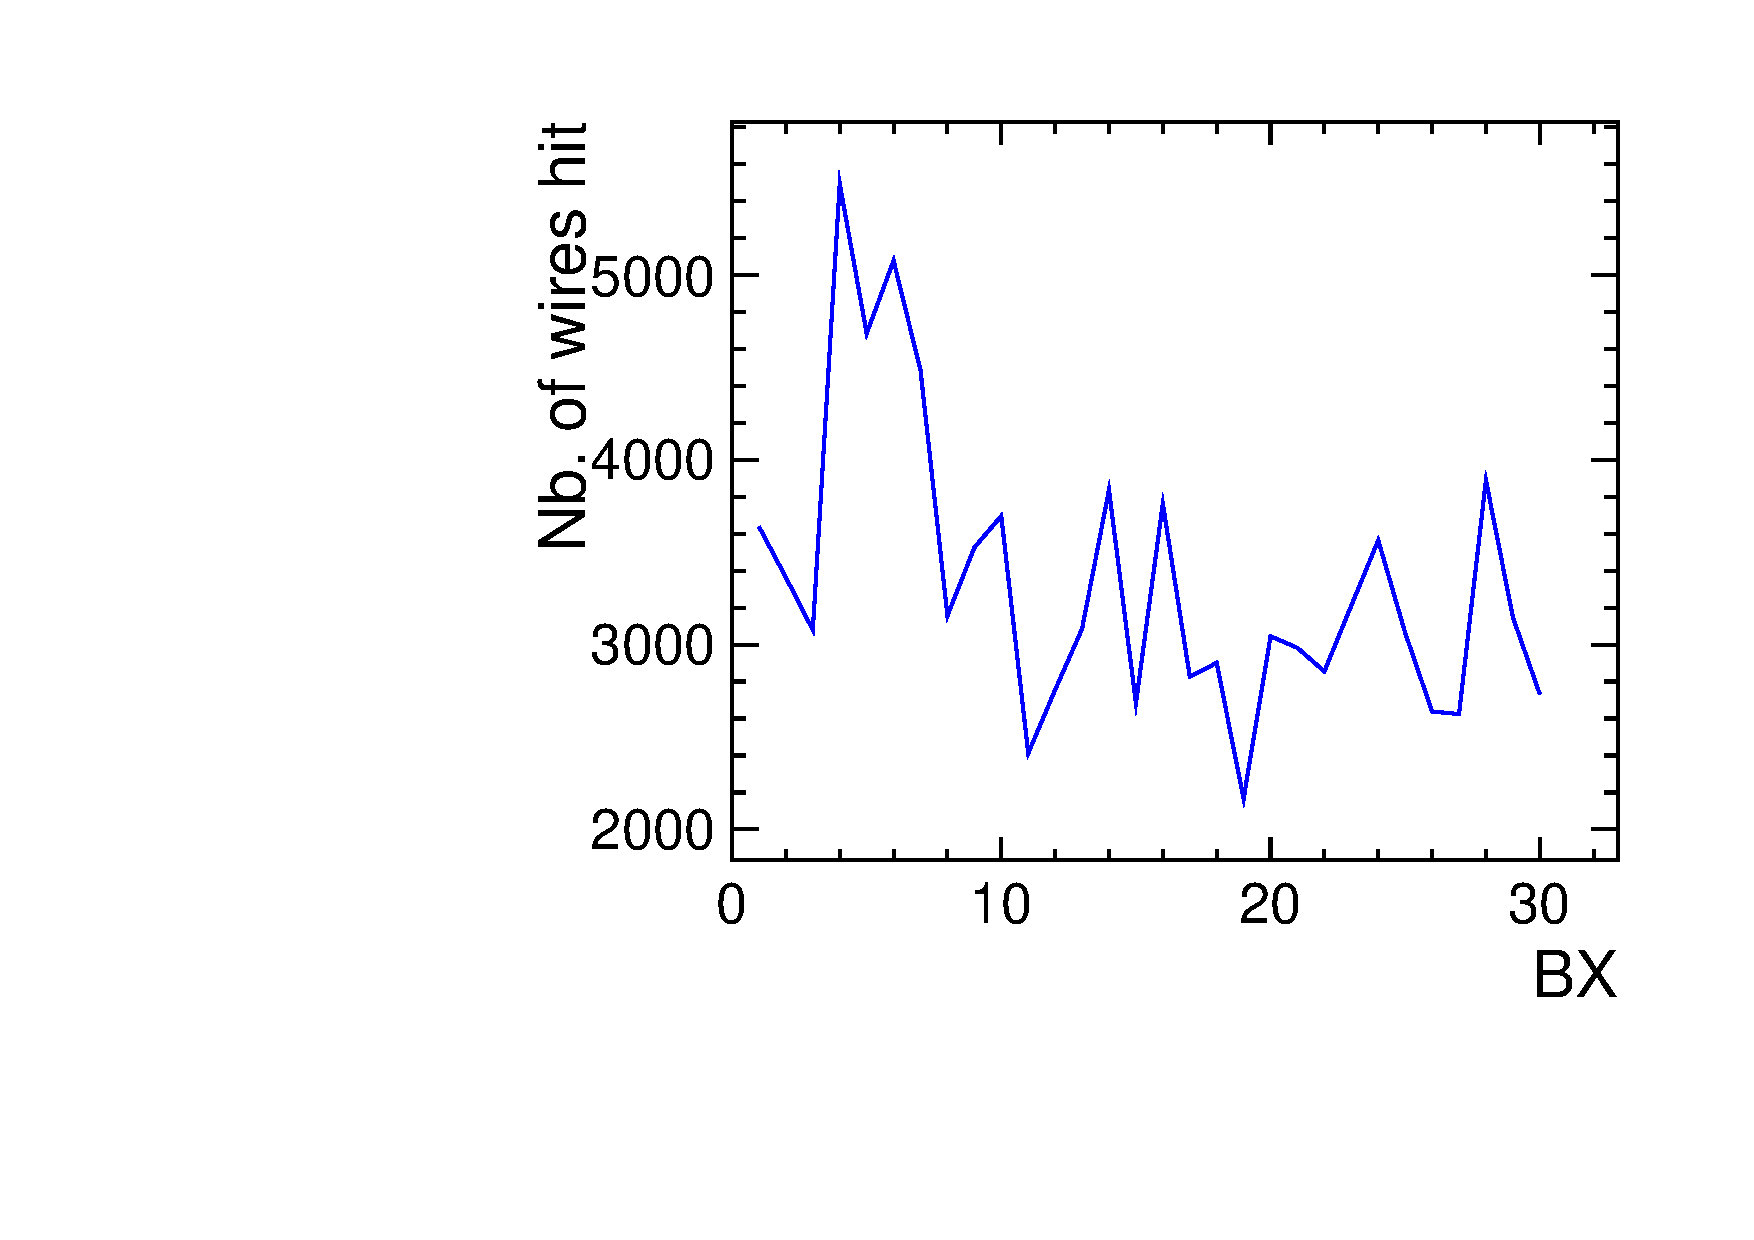
\includegraphics[width=\textwidth]{../figures/DCH/differentWires_hit_perBX.pdf}

	\end{columns}
	
\end{frame}

%%%%%%%%%%%%%%%%%%%%%%%%%%%%%
%         SLIDE             %
%%%%%%%%%%%%%%%%%%%%%%%%%%%%%
\begin{frame}
	\frametitle{Background hits in the DCH}

	\begin{columns}
	\column{0.5\textwidth}
	\centering
       \begin{itemize}
         \item Hits due to the background  \vspace{0.2cm}
          \begin{itemize}
          \item Loopers
          \item Tracks in the forward region \vspace{1cm}
		\end{itemize}       
       
        \item Pattern recognition possible for occupancy levels of: \vspace{0.2cm}
          \begin{itemize}
          \item $20\%$ for inner-most layers
          \item $5\%$ for outer-most layers \vspace{0.2cm}
          \end{itemize}

        \end{itemize}


	\column{0.5\textwidth}	
	\centering
        \begin{tikzpicture}
          \node[anchor=south west,inner sep=0] (image) at
          (0,0){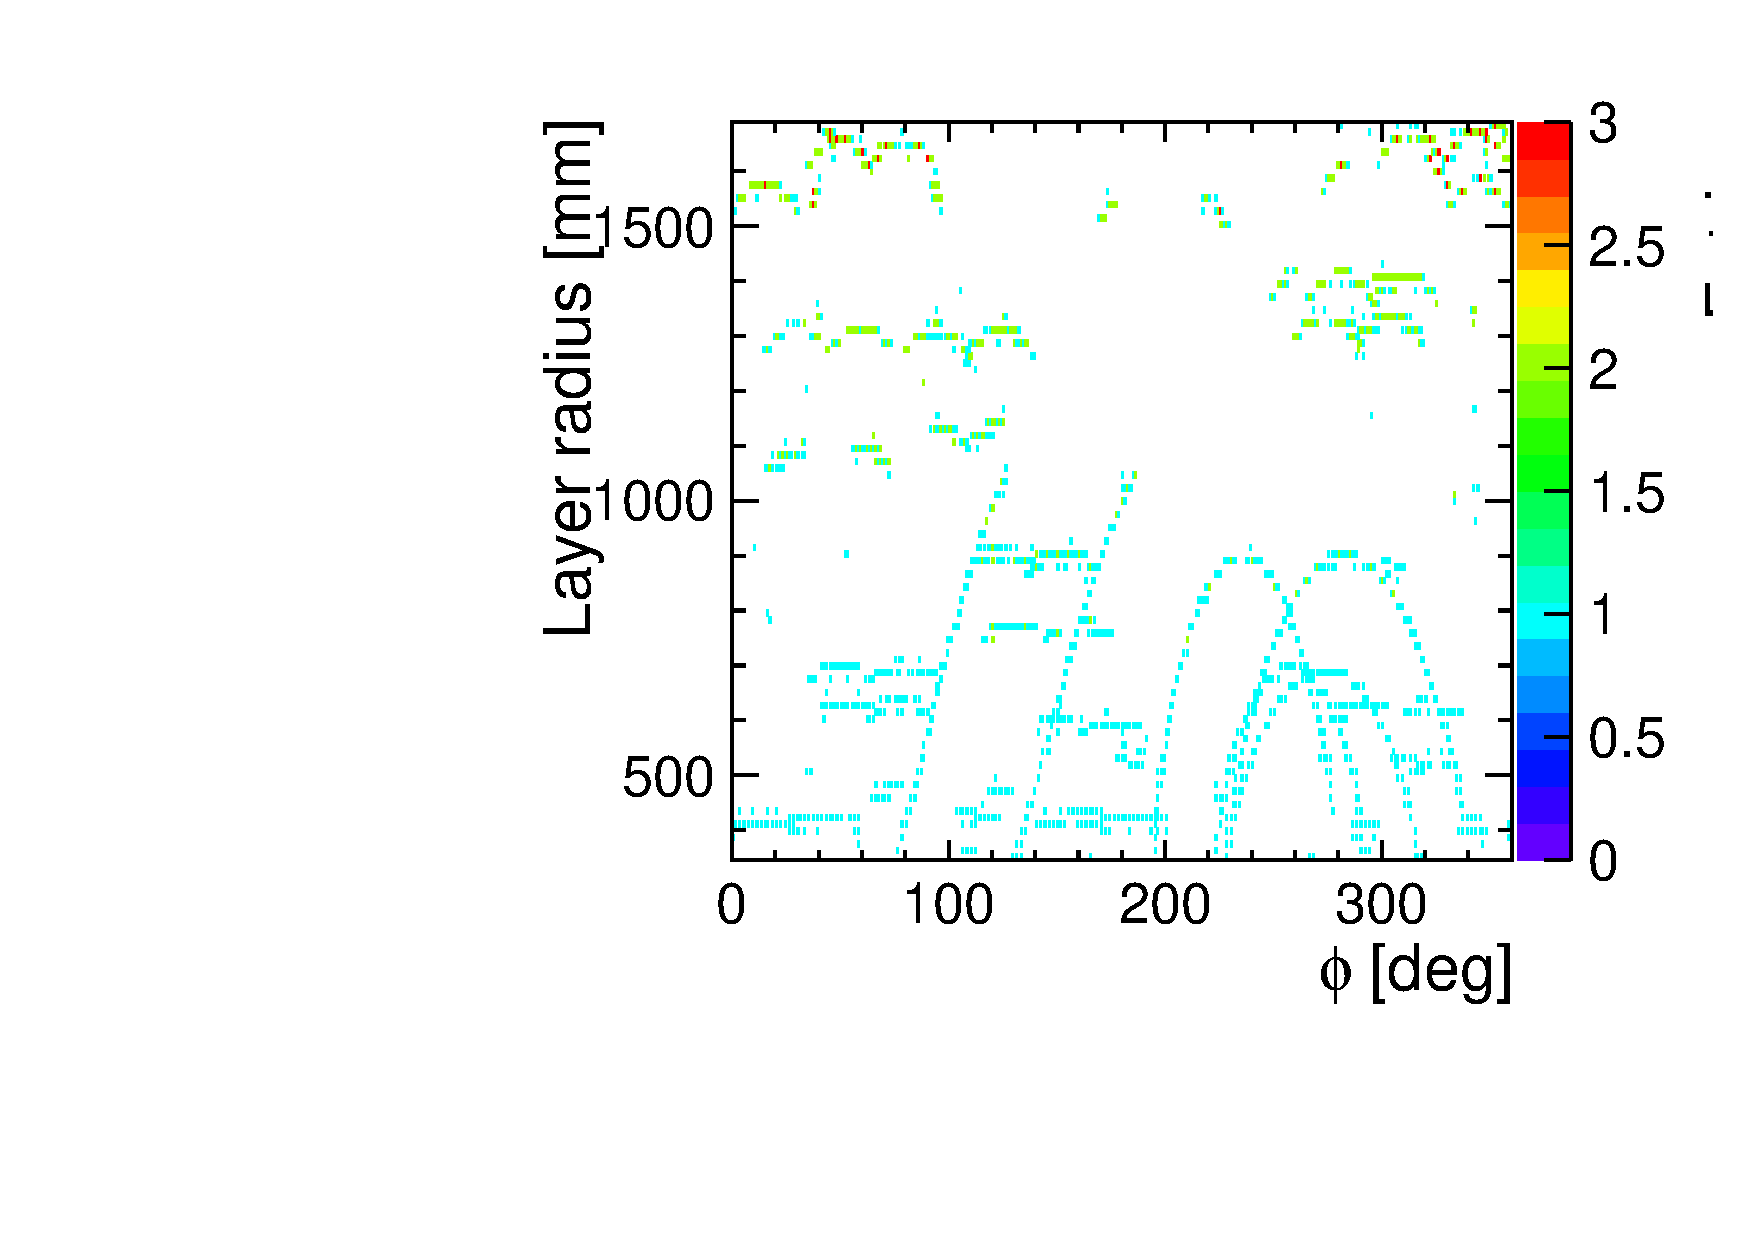
\includegraphics[width=\textwidth]{../figures/layerR_vs_phi.pdf}};
          \begin{scope}[x={(image.south east)},y={(image.north west)}]

            % \draw[help lines,xstep=.1,ystep=.1] (0, 0) grid (1,1);
            % \foreach \x in {0,1,...,9} { \node [anchor=north] at (\x/10,0) {0.\x}; }
            % \foreach \y in {0,1,...,9} { \node [anchor=east] at (0,\y/10)
            % {0.\y}; }
            % 
            \node[above] at (0.5, 0.8) {\textcolor{red}{Work in progress}}; 
            
          \end{scope}
        \end{tikzpicture}
	\end{columns}
	
\end{frame}

%%%%%%%%%%%%%%%%%%%%%%%%%%%%%
%         SLIDE             %
%%%%%%%%%%%%%%%%%%%%%%%%%%%%%
\label{lastslide}
\begin{frame}
  \frametitle{Summary \& Outlook}
  
  	\vspace{1cm}
	\begin{itemize}
	\item Full simulation of the FCCee-IDEA detector concept with FCCSW
	\item Implementation of the drift chamber 
		$\Rightarrow$ geometry, segmentation, simulation \& reconstuction
	\item Validations done and still ongoing 
	\item First physics studies:
		\begin{itemize}
		\item Impact of beam-induced backgrounds: $e^{+}e^{-}$ pairs from $\gamma\gamma$ collisions
	  	\item Estimation of the occupancy in the VXD and DCH with FCCSW and comparison with ILCSoft
	  	\item More investigation on the occupancy is needed for the DCH to draw final conclusions
	  	\end{itemize} \vspace{0.2cm}
	\item Future work:
		\begin{itemize}
		\item Implementation of a realistic material around DCH 
		\item Study the effect of other beam-induced
                  backgrouds (the synchrotron radiation \& $\gamma\gamma\rightarrow$~hadrons)
		\item Track reconstruction in FCCSW
		\end{itemize}
  	\end{itemize}

	\vspace{0.5cm}
	\centering
	\Large{\textbf{Thank you for your attention!}}
\end{frame}

%%%%%%%%%%%%%%%%%%%%%%%%%%%%%
%         SLIDE             %
%%%%%%%%%%%%%%%%%%%%%%%%%%%%%
\begin{frame}

	\centering
	\Huge{Backup slides}
\end{frame}

%%%%%%%%%%%%%%%%%%%%%%%%%%%%%
%         SLIDE             %
%%%%%%%%%%%%%%%%%%%%%%%%%%%%%
\begin{frame}
	\frametitle{Impact of incoherent pairs in the DCH}

	\begin{itemize}
	\item Number of wires hit as a function of the layer radius
	\end{itemize}

	\begin{columns}
	\column{0.5\textwidth}
	\centering
	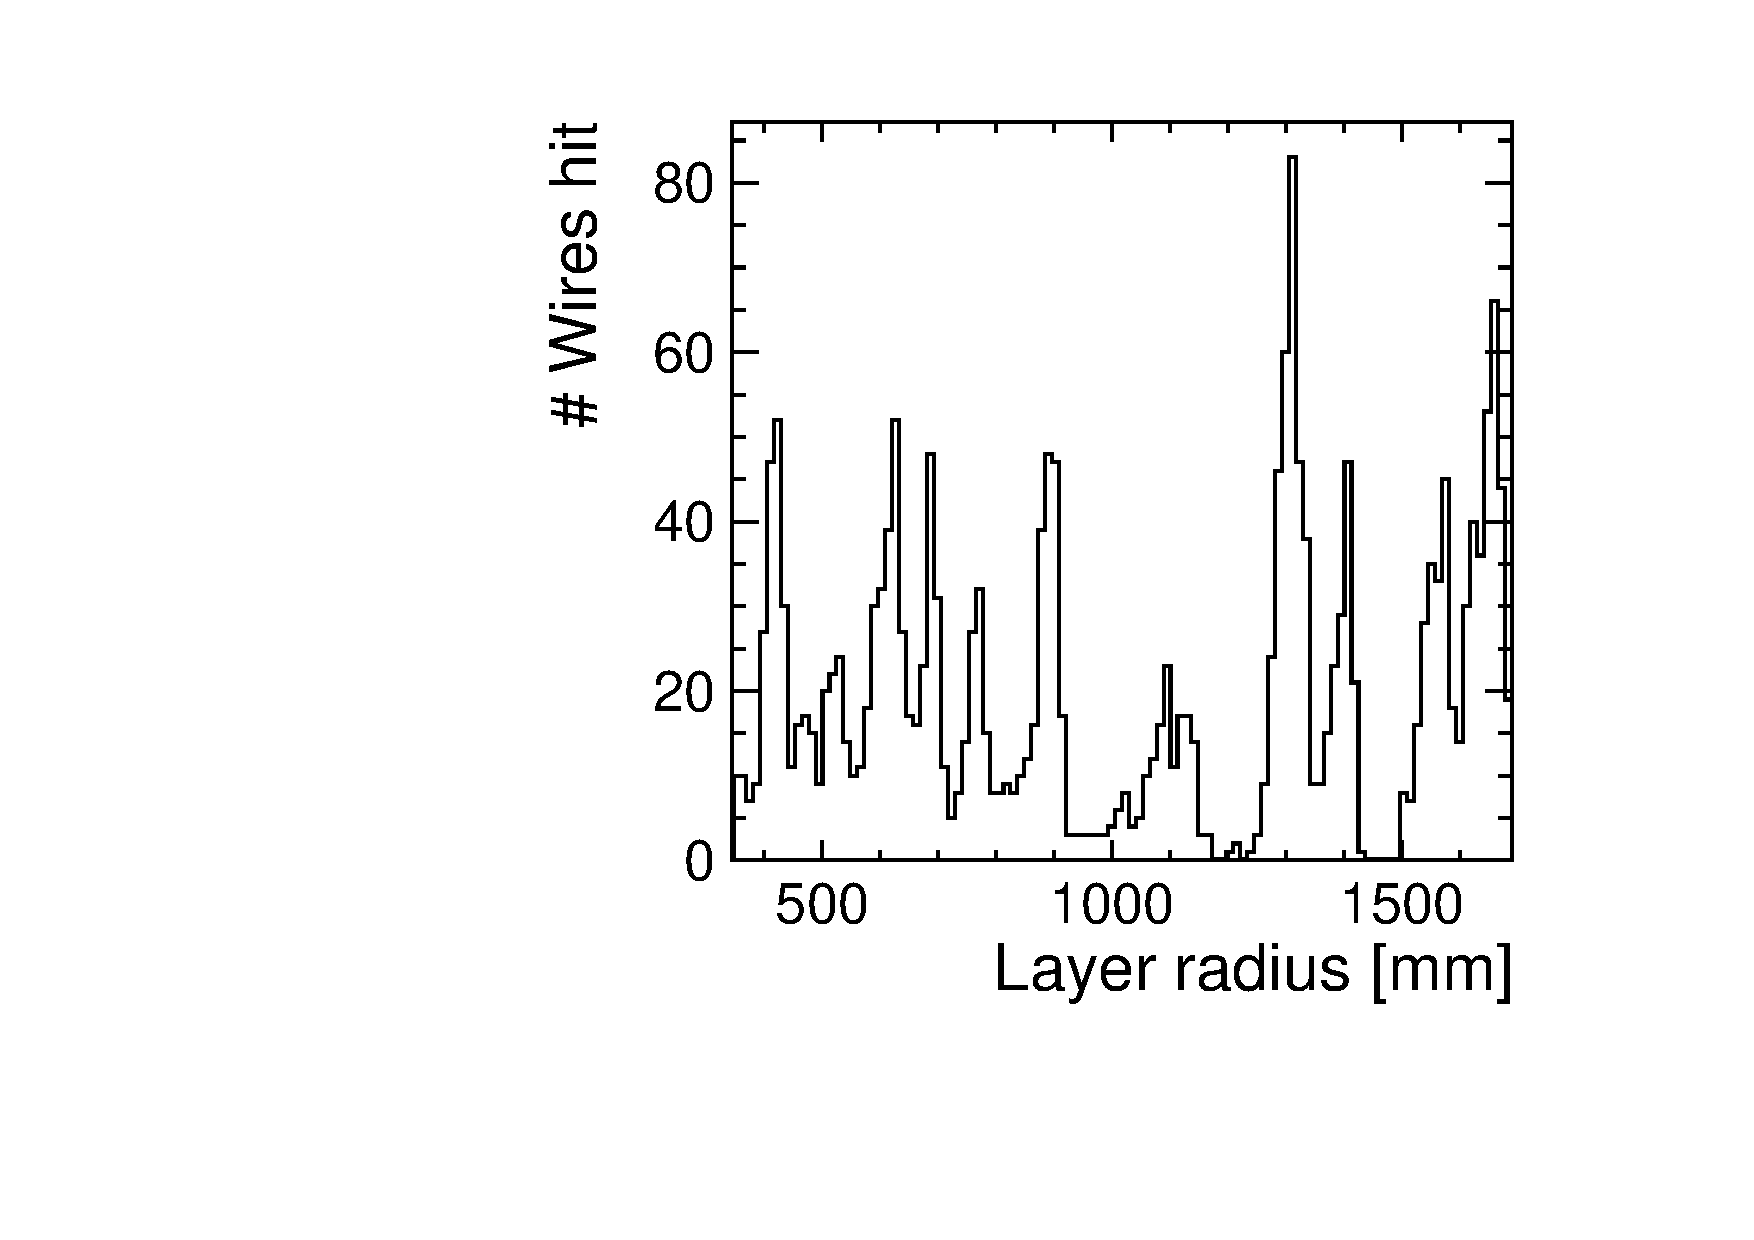
\includegraphics[width=\textwidth]{../figures/layerR_vs_wires.pdf}

	\column{0.5\textwidth}	
	\centering
	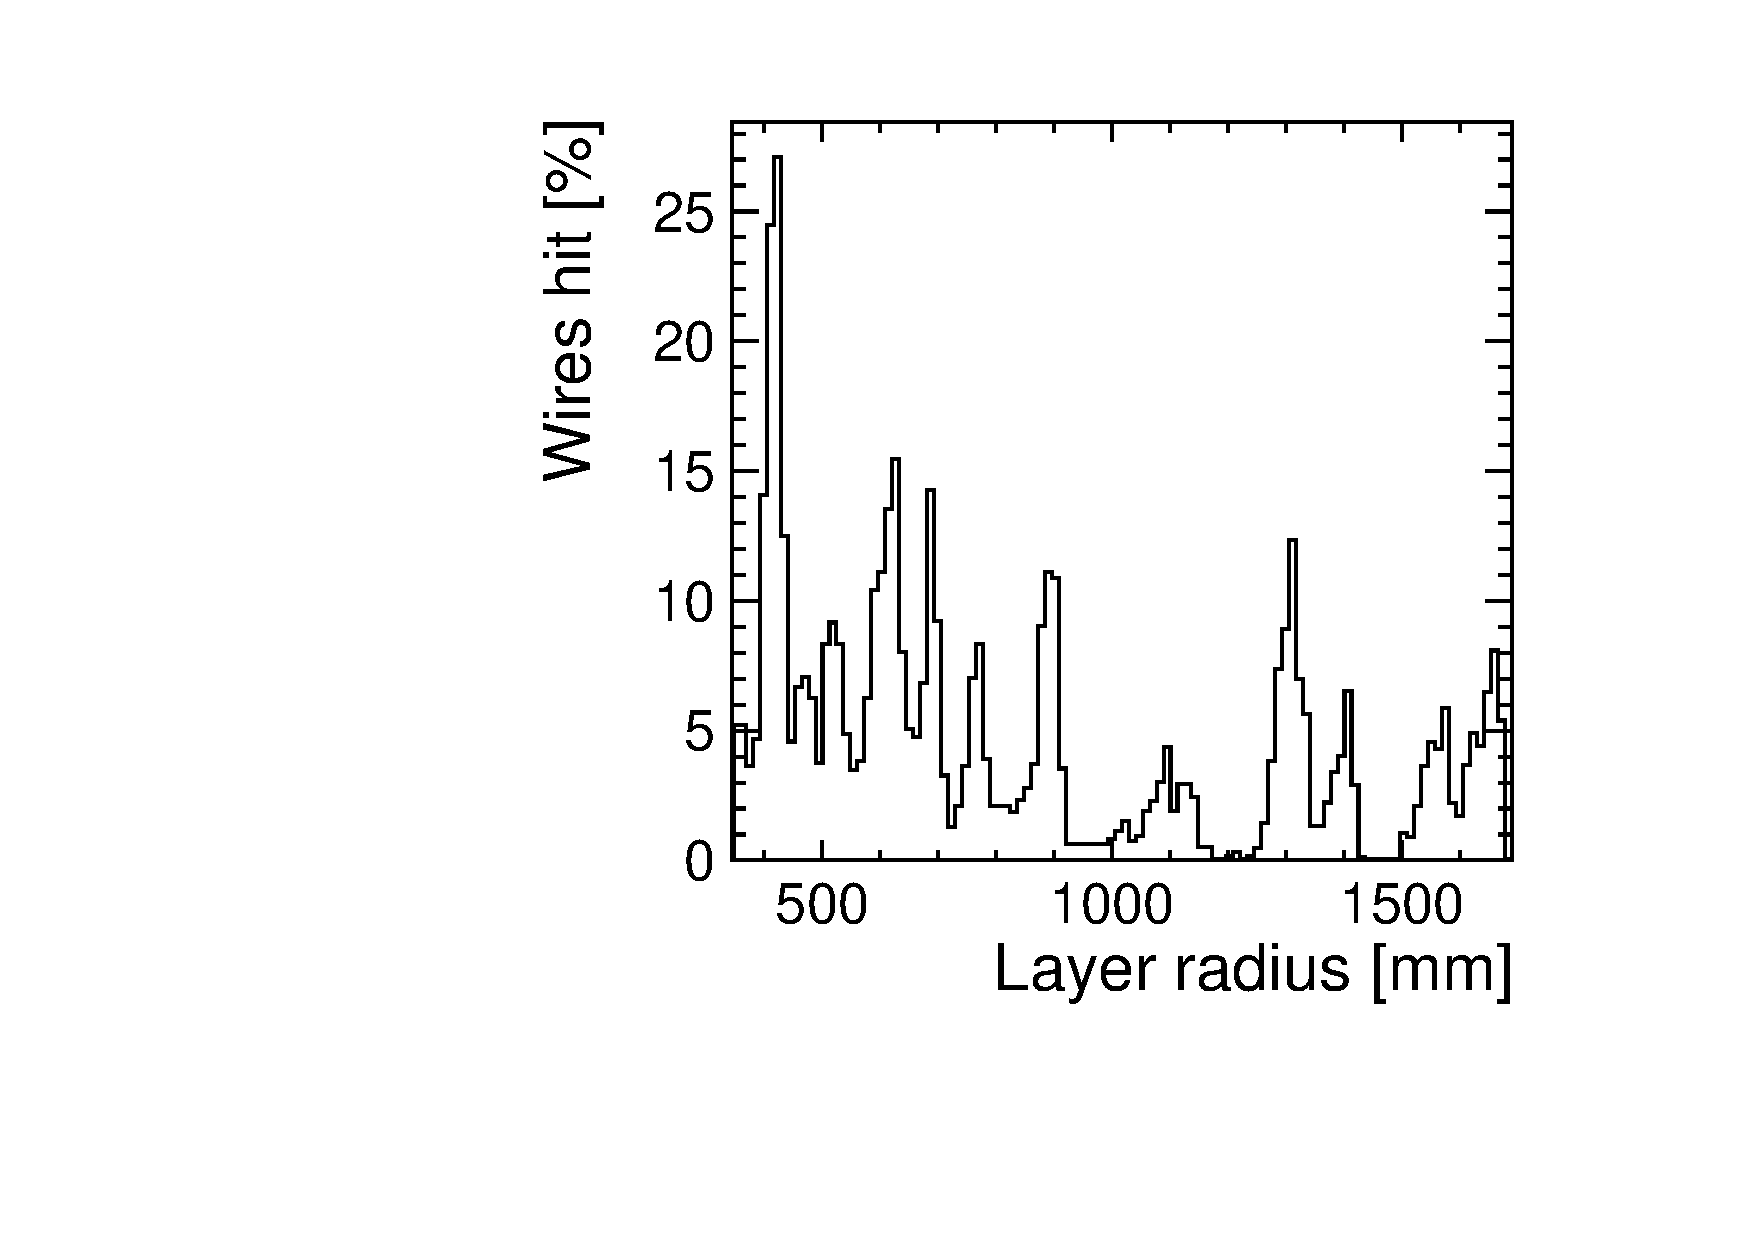
\includegraphics[width=\textwidth]{../figures/layerR_vs_wires_percent.pdf}	
	
	\end{columns}
	
\end{frame}

%%%%%%%%%%%%%%%%%%%%%%%%%%%%%
%         SLIDE             %
%%%%%%%%%%%%%%%%%%%%%%%%%%%%%
\begin{frame}
	\frametitle{Secondary vertices produced}


	\centering
	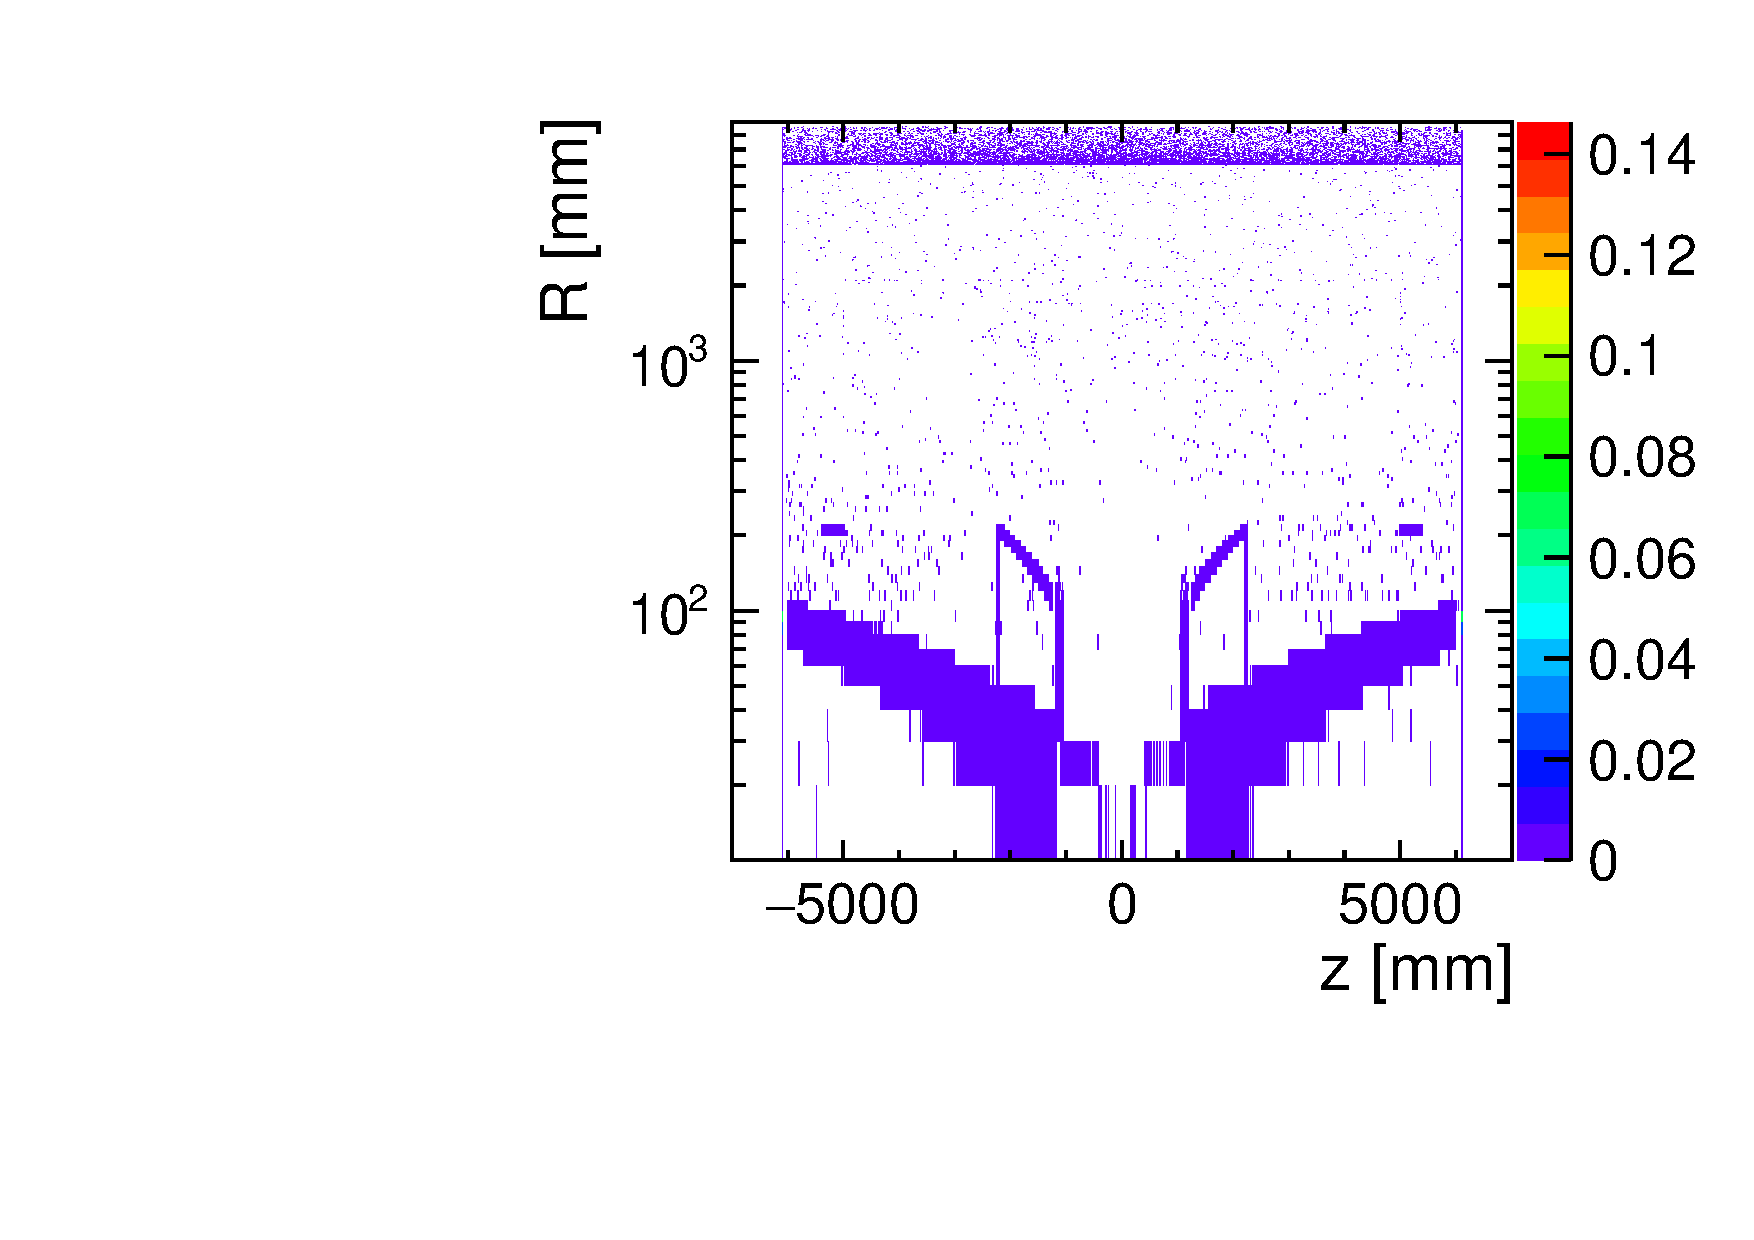
\includegraphics[width=0.7\textwidth]{../figures/SecondaryVertices_logScale.pdf}

	
\end{frame}



%----------------------------------------------------------------------------------------
%	End of Document
%----------------------------------------------------------------------------------------
\end{document} 
